
\chapter{Etapas propostas no Plano de Trabalho}
As etapas do plano de trabalho buscou direcionar as atividades de pesquisa de modo que a cada passo o bolsista conseguisse formar uma base sólida de entendimento da sua área de pesquisa. A fim de alcançar os objetivos do Projeto de Pesquisa as etapas a seguir foram estipuladas:
\begin{enumerate}
    \item  Estudo bibliográfico das perspectivas nacional e internacional no que diz respeito a veículos autônomos;
    \item  Pesquisa bibliográfica para compreender o que busca economicamente e tecnologicamente o mercado internacional e nacional em relação a veículos autônomos;
    \item Aprender quais são os diferentes tipos de veículos autônomos;
    \item Pesquisa bibliográfica das tecnologias essenciais de um carro autônomo;
    \item Mapear e entender os principais softwares de controle de um carro autônomo;
    \item Elaboração do Relatório Final.
\end{enumerate}

No decorrer desse ano de pesquisas foi possível desenvolver, de forma satisfatória, todas as etapas do projeto. Contudo, a etapa 5 devido a sua grandiosidade necessita de uma pesquisa única e mais aprofundada. De modo a aprofundar e consolidar os conhecimentos do bolsista na área de software para a direção autônoma.

\newpage
\chapter{Objetivos}\label{Objetivos}
\section{Objetivo Geral}\label{Objetivo Geral}
Neste primeiro ano, os nossos objetivos foram documentar e entender o cenário de Veículos Autônomos no mundo e nesse processo contrastar com o brasileiro. De modo, a compreender o cenário automobilístico e suas expectativas para essa categoria de veículos. Portanto, foi buscado identificar as principais diferenças entre esses veículos e o que se espera economicamente e tecnologicamente dessa tecnologia, tanto para o Brasil e o mundo. Por fim, mapeamos quais são os principais recursos tecnológicos que fazem esses veículos possíveis. 

\section{Objetivos em Específico}\label{Objetivos Específicos}
\begin{enumerate}
    \item  Entender o cenário de Veículos Autônomos no mundo, e contrastar com o brasileiro:
    \begin{enumerate}
        \item Compreender o cenário automobilístico brasileiro, e as suas expectativas para essa tecnologia.
        \item Contrastar o mercado de veículos autônomos mundial com o brasileiro, buscando  decifrar o que é necessário para a aplicação dessa tecnologia no país.
    \end{enumerate}
    \item  Estudar as principais empresas de pesquisa que trabalham com Veículos Autônomos no mundo, e o que buscam economicamente e tecnologicamente no setor:
    \begin{enumerate}
        \item Identificar se buscam diferentes tipos de Carros Autônomos. Assim como entender as suas possíveis principais diferenças.
        \item Entender o que essas empresas buscam alcançar economicamente, e tecnologicamente ao inserir essa tecnologia no mercado.
        \item Conhecer as mudanças econômicas que carros autônomos podem trazer para a sociedade brasileira. 
    \end{enumerate}
    \item Mapear as tecnologias essenciais para a Direção Autônoma:
    \begin{enumerate}
        \item Documentar quais são os Softwares, algoritmos de controle, e sensores usados nesses veículos.  
    \end{enumerate}
\end{enumerate}

\newpage
\chapter{Metodologia}
Utilizamos uma metodologia, com o fim de revisar a literatura existente, que tem como essência desenvolver e colocar o bolsista em contato direto com todo material já desenvolvido em relação a esta iniciação científica, constituído principalmente de: artigos científicos, cursos online, publicações em periódicos, jornais online, monografias e dissertações.

Nesse formato metodológico, pesquisa bibliográfica, foi possível ter contato e se fundamentar com os principais materiais da atualidade relacionados a veículos autônomos. De modo a ter contato com o que há de mais recente sobre o assunto.

Ressaltamos que, com o decorrer das pesquisas, foram encontradas fontes relevantes, que já possuem mais de 3 anos desde sua publicação. Devido a isso, o bolsista tomou essas publicações como ponto de partida para atualizar-se sobre o que há de mais novo sobre o assunto, de maneira a sempre manter o conteúdo deste relatório o mais atual possível.

A pesquisa bibliográfica seguiu as seguintes etapas \cite{bibli}: 

\begin{figure}[H]
\centering
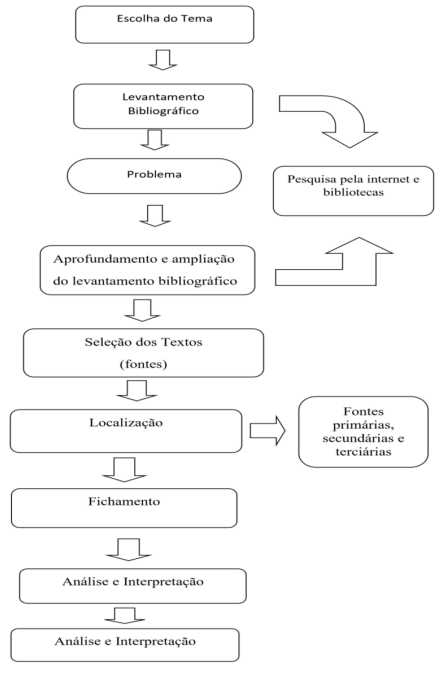
\includegraphics[width=8cm]{Figures/bibli.png}
\caption{Etapas da pesquisa Bibliográfica.}
\label{img_bibli}
\end{figure}

As etapas apresentadas acima foram seguidas pelo bolsista de modo a auxiliá-lo na
delimitação do tema a ser pesquisado e em sua organização.

\vspace {1cm}


A seguir forneceremos detalhamento para as etapas (Figura \ref{img_bibli}) da pesquisa bibliográfica desenvolvida neste projeto:

\vspace {1mm}


\begin{itemize}

\item \textbf{Escolha do tema:} A escolha do tema foi feita no desenvolvimento do Plano de Trabalho para essa Iniciação Científica; Veículos Autônomos e suas tecnologias. 

\item \textbf{Levantamento Bibliográfico:} O bolsista fez o seu levantamento preliminar através dos seguintes meios na internet (Google academic, Google livros, biblioteca virtual, bibliotecas, site das bibliotecas de universidades, CAPES e outros). Foram pesquisadas referências na plataforma scholar.google.com, no portal do Periódico CAPES, e jornais e artigos pela internet. A busca nos bancos de dados abrangeu os anos de 2022 a 2023. Contudo, a partir de pesquisas na internet, também, fizemos uso de materiais publicados a partir de 2019. Como palavra-chave utilizou-se os termos: Autonomous Vehicles, Autonomous, Cars, Mobility, Connected Car, AV, TaxiBot, e self-driving cars.  A pesquisa limitou-se nos idiomas inglês, português,  alemão, e espanhol (Por ordem de uso).


\item \textbf{O problema:} Devido ao enquadramento dessa pesquisa, por visar unicamente o enriquecimento do bolsista sobre os materiais já desenvolvidos sobre o tema. Este trabalho não busca responder, necessariamente, a um problema de pesquisa. Devido a isso, podemos enquadrar nossos Objetivos (seção \ref{Objetivos}) nessa etapa, de modo a ser nossa estrela guia para desenvolver a pesquisa.

\item \textbf{Aprofundamento e ampliação do levantamento bibliográfico:} Buscamos por obras (artigos, teses, matérias) mais recentes, dos últimos 3 anos, para nos mantermos atualizados evitando conteúdos obsoletos. Mantivemos um número razoável de fontes bibliográficas, de modo que o bolsista não se perdesse durante o desenvolvimento de sua pesquisa. 

\item \textbf{Seleção das fontes:} Houve a seleção das fontes mais relevantes para o projeto. para seleção dos artigos, o primeiro filtro ocorreu pela leitura dos seus títulos, sendo selecionados os que se referiam as palavras-chave. A segunda filtragem foi realizada a partir da leitura dos resumos (abstracts). Neste filtro foi possível identificar publicações que apresentaram relevância para o nosso tema.
Portanto, por meio de uma leitura crítica o bolsista buscou assimilar as obras levantadas, sempre analisando se faria sentido usá-las para o desenvolvimento do projeto. 

\item \textbf{Localização das fontes:} Como apresentado na etapa de  \textit{Levantamento Bibliográfico} estaremos fazendo uso de recursos online para este projeto. Sobretudo, da plataforma CAPES.

\item \textbf{Fichamento:} Para este projeto não foi realizada a classificação dos artigos encontrados. Entretanto, nessa etapa, foram feitos resumos de modo a auxiliar o bolsista no firmamento de seus conhecimentos, e no desenvolvimento deste relatório final.

\item \textbf{Análise e Interpretação:} Buscamos averiguar se os materiais encontrados contém valor teórico para o projeto, se sofreu alterações, interpolações, e possíveis falsificações ao longo do tempo. Houve, também, a checagem das fontes dos materiais apresentados, de modo a sempre buscar pela fonte principal do assunto, e nos principais meios de mídias globais.


\end{itemize}

 
Como apresentado no plano de trabalho, a Iniciação Científica buscou seguir um princípio metodológico “Project-based learning” \cite{krajcik2006project}, que visa construir soluções a partir de problemas reais em nossa sociedade. Visto que, é uma modalidade de estudo que deixa as pessoas envolvidas livres para seguir a sua curiosidade, desejo de resolver os problemas encontrados pelo caminho e de buscar por mais informações para resolvê-los, contempla os objetivos desejados para a realização de maneira satisfatória deste projeto. 

Além disso, as pesquisas fundamentam-se no método de pesquisa Revisão Sistemática de Literatura (RSL) que segundo Maria Cristiane \cite{revi3}, e Nakano \cite{revi2} refere-se a um tipo de investigação que se concentra em uma questão bem definida, visando identificar, selecionar, avaliar e sintetizar as evidências disponíveis relacionadas a uma questão formulada de interesse para o pesquisador, esse princípio e método foram utilizados nas etapas definidas na figura \ref{img_bibli} .

Por fim, enaltecemos que devido ao formato de pesquisa, as fontes do bolsista foram crescendo com o passar do tempo e de suas pesquisas. Portanto, o seu levantamento bibliográfico encontra-se muito mais rico comparado com o início de sua seleção bibliográfica.


\vspace {1cm}

O bolsista, também, utilizou dos seguintes formatos de aprendizado durante o desenvolvimento do projeto.
\begin{itemize}
\item \textit{Cursos e minicursos;}
\item \textit{Participação em eventos.}
\end{itemize}


\subsection{Veículos Autônomos no Brasil e no mundo}

\subsection{Veículos Autônomos e suas perspectivas}

\subsection{Tecnologias Essenciais para a Direção Autônoma}

\newpage

\chapter{Resultados e Discussão} \label{resultados}

\section{Veículos Autônomos no Brasil e no mundo}

\subsection{to do}


\subsection{Implementação de Veículos Autônomos no Brasil e no Mundo}

Antes de entendermos como implementá-lo, precisamos entender quais são esses veículos: Veículos autônomos são todos os veículos que não exigem um motorista humano de maneira parcial ou total para conduzi-los, ou seja, veículos que podem dirigir sozinhos. Alguns veículos que podem ser considerados autônomos já fazem parte do cotidiano de certas cidades, são os metrôs e trens que não precisam de motorista, ou o motorista só está ali para casos extremos. No entanto, com os últimos avanços e inovações tecnológicas, a automação está se expandindo não apenas para trens, mas também para carros, caminhões, ônibus, escavadeiras (entre outros veículos industriais) e até barcos, navios e aviões. Com a automação desses meios de transporte, o mundo experimentará uma reviravolta sem precedentes \cite{4cenarios_ocidental}.

Nesse aspecto, o estudo de sua implementação, a ser desenvolvido nos próximos subcapítulos, é fundamental para compreendermos quais âmbitos da nossa sociedade essa categoria de veículos terrestres podem ser alocados, e os benefícios e dificuldades de sua implementação no Brasil e no mundo.

 \subsubsection{Expectativas com a implementação dos Veículos Autônomos}
Devido ao seu potencial transformativo, vários benefícios são esperados. Entre esses benefícios e expectativas estão o de redução de acidentes de trânsito. Estima-se que no brasil o número de mortes em acidentes de transporte terrestre no período de 2019 foi de 31.945 \cite{Anexo_I_pnatrans}. Veículos autônomos vêm com a promessa de buscar uma redução nesses números através da retirada do principal causador de acidentes de trânsito: erros humanos. 

Ademais, Veículos Autônomos vem como uma forma de minimizar os congestionamentos nas grandes metrópoles. Segundo o  Plano Estratégico de Desenvolvimento Urbano Integrado da Região Metropolitana do Rio de Janeiro, \cite{rj_transito}, apenas na hora do rush da manhã o fluxo de viagens de São Gonçalo a Niterói chega a quase 100 mil pessoas sendo transportadas; desses deslocamentos cerca de 80\% das viagens são feitas em transporte público – ônibus convencionais. Diante disso, uma das propostas para suprir essa demanda de transporte seria a inclusão de veículos autônomos. Nesse formato, carros poderiam ser solicitados como, hoje, são feitas as corridas de aplicativos, e os ônibus do transporte público  poderiam operar por mais horas e com menor custo. 
Entretanto, ainda seria necessário lidar com outros problemas como a disputa de espaço nas vias, e os engarrafamentos crônicos das cidades; De acordo com informações do levantamento domiciliar realizado durante a elaboração do último PDTU, o tempo médio de deslocamento do centro de São Gonçalo a Niterói é de 50 minutos, devido a problemas relacionados ao grande fluxo de veículos, sendo o transporte público quase 25\% maior. Diante disso, os veículos autônomos teriam que disputar espaço nas vias com veículos ainda conduzidos por pessoas. Sabendo que essa categoria será e está sendo implementada de maneira gradual na sociedade, começando por veículos de luxo \cite{caio}.

\begin{figure}[H]
\centering
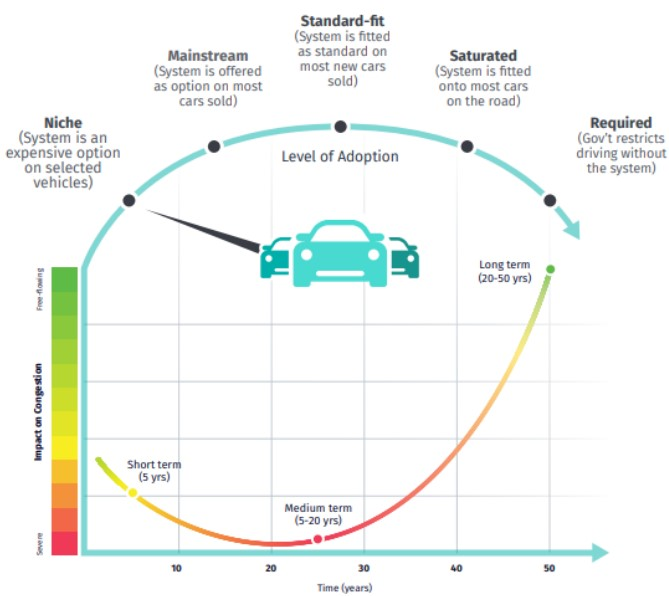
\includegraphics[width=10cm]{Figures/conge.jpg}
\caption{Impacto dos níveis de autonomia no congestionamento ao longo do tempo \cite{4cenarios_ocidental}.}
\label{congestionamento}
\end{figure}

Um estudo de casos considerado um cenário onde veículos autônomos têm que lidar com congestionamentos, levaram à conclusão de que o aumento do número de veículos autônomos, totalmente conectados, dirigindo em pelotões dentro de uma rede, reduz os atrasos e congestionamentos. Como resultado, mantém ou melhora o tráfego da rota escolhida no estudo. O veículo líder do pelotão foi capaz de antecipar mudanças nos sinais e comunicá-los com os veículos de trás, permitindo-lhes um melhor desempenho em cruzamentos sinalizados. Os pelotões também aumentaram a capacidade de rede em links congestionados, permitindo melhor desempenho nos atrasos médios \cite{conge}.

\subsubsubsection{Implementação em setores industriais}

Ainda tratando sobre benefícios em veículos
autônomos em nossa sociedade.
Há a utilidade dessa categoria em ambiente industrial, onde poderiam  operar em indústrias automotiva, indústria de bebidas, indústria eletroeletrônicas, implementos agrícolas, porto, linha de montagem, almoxarifado, etc.

A aplicação de veículos autônomos em portos é uma solução que visa aumentar a eficiência do transporte de contêineres e materiais para os navios e setores de portos. O uso desses veículos aumenta a automação de movimentação logística, acelerando o processo de carga, descarga e armazenamento de carga. Fazendo com que a produção tenha um ganho significativo 
na competitividade do mercado, aumento da produtividade e redução de custos das indústrias, na qual esforçar-se para otimizar os processos de manuseio de materiais por meio da automação, essas máquinas podem atuar de maneira ótima em rotas programadas tanto na função de abastecimento nas linhas de produção quanto na transferência entre estações ou áreas do processo produtivo e no transporte de matéria-prima ou produto acabado \cite{aplicacao}.

\subsubsection{Veículo Autônomo e áreas de implementação} \label{implementacao}

Devido a sua simplicidade, segurança e conforto em operação. Podem ser aplicados em diversas áreas e setores da sociedade, como na execução de funções e tarefas de risco que  seres humanos não seriam capazes de realizar, ou na execução de funções exaustivas, onde o ser humano teria uma menor eficiência. Visto que a maioria desses veículos  tem suas funções executadas automaticamente necessitando de nenhum ou pouca supervisão de um humano. 
Os tornando perfeitos, também, para pessoas com deficiência e idosos viverem suas vidas de forma mais independente. 
\vspace {1cm}

Aplicações especializadas de veículos autônomos \cite{aplicacao2}:

\begin{enumerate}
 \item \textbf{Transporte público:} O Veículo Autônomo (VA) foi introduzido inicialmente no sistema de transporte público na modalidade de operação sem condutor. Hoje em dia, as tendências modernas no transporte público são úteis na região metropolitana para os turistas, próprios cidadãos, etc. Como visto, o transporte é um grande desafio em áreas lotadas, apertadas e desordenadas em várias cidades. Ainda assim, devido à introdução de veículos elétricos autônomos, é possível gerenciar os problemas em locais congestionados. Como mencionado anteriormente, um dos benefícios do trânsito sem motorista seria o melhor serviço para passageiros com deficiência. O serviço de transporte para pessoas com deficiência geralmente é inconveniente, não confiável e caro. Os passageiros com deficiência geralmente precisam reservar uma viagem 24 horas antes da partida e são informados de que a coleta pode ocorrer a qualquer momento durante uma janela de 2 horas \cite{notif}.
\item \textbf{Bonde e Trem Elétrico Autônomo:} O primeiro veículo sobre trilhos elétrico automatizado foi projetado e desenvolvido pela Siemens na Alemanha. Em 2018, o primeiro test drive do bonde foi realizado na Alemanha por sete quilômetros. O uso de dispositivos inteligentes, como câmeras inteligentes, sensores inteligentes e sistemas LiDAR inteligentes baseados em software, é útil para o bonde dirigir em áreas lotadas de várias cidades sem nenhum obstáculo. Devido ao algoritmo inteligente, sistemas inteligentes de monitoramento e controle, um bonde operará com segurança mesmo em áreas lotadas. Diante de qualquer obstáculo, o bonde se encarregará de solucionar a situação com o auxílio de outros aparelhos auxiliares, iniciando-se o trajeto imediatamente após a retirada do obstáculo do seu caminho. Nesse mesmo sentido, houve o Harry projetado e desenvolvido em 2017, na Inglaterra.Visando suprir a falta de transporte público em algumas localidades de Londres.
\item \textbf{Helicóptero Elétrico Autônomo:} O VSR700 é um dos protótipos inovadores de Helicópteros Elétricos Autônomos inventados em 2020 pela Airbus em um teste pesado na França. Ele é projetado e desenvolvido para operar ao lado de vários meios navais. O objetivo é fortalecer os navios, aumentar seu escopo usando sensores inteligentes em associação com helicópteros e aprimorar o cenário de coleta de informações das perspectivas do navio. Os Helicópteros Autônomos estão fazendo o trabalho de vigilância das informações de seus alvos e confirmando o destino de chegar aos navios nos locais desejados. 
\item \textbf{Caminhão Inteligente Autônomo:} Um caminhão elétrico totalmente automatizado foi projetado e desenvolvido em 2016 com o nome Otto. Sem motorista humano, opera com a ajuda do sistema LIDAR. Esses caminhões modernos minimizam os acidentes e são utilizados para entrega de mercadorias e serviços pesados. Além disso, o caminhão elétrico autônomo Vera, um Volvo, foi projetado e desenvolvido para transportar mercadorias de diversos destinos, como indústrias, estaleiros, minas, portos, pátios de armazenamento e armazéns e possui formas muito eficientes, seguras, limpas e sustentáveis do que os caminhões atuais mais comuns.

\item \textbf{Veículo Subaquático Autônomo:} É usado em estudos geográficos da marinha e também é popular no setor técnico e de defesa. A principal função deste veículo é obter uma imagem aprimorada do fundo do mar com uma resolução muito alta da superfície de uma embarcação, ou objeto de investigação.
\item \textbf{Veículos Autônomos para Agricultura e Mineração:}  Os veículos autônomos são usados no setor agrícola para vários processos agrícolas e usados em tarefas operacionais de mineração. Diferentes tipos de veículos autônomos de agricultura e mineração são tratores agrícolas autônomos, veículos terrestres não tripulados usados para fazendas inteligentes, veículos de mineração, como caminhões de mineração, máquinas automatizadas de mineração, etc.

\end{enumerate}

\subsection{O cenário de aplicação de Veículos Autônomos}
Segundo o relatório “2020 Autonomous Vehicles Readiness Index” da KPMG; empresa que opera em 143 países e territórios em todo o mundo, oferecendo serviços de auditoria, impostos e consultoria. Este relatório buscou avaliar a preparação de 30 países e jurisdições na corrida por veículos autônomos, sendo uma ferramenta para ajudar a medir o nível de preparação para veículos autônomos. É um índice composto que combina 28 medidas individuais de uma variedade de fontes em uma única pontuação. Mais informações sobre os resultados, metodologia e fontes utilizadas podem ser encontradas em, \cite{KPMG}.

\begin{figure}[H]
\centering
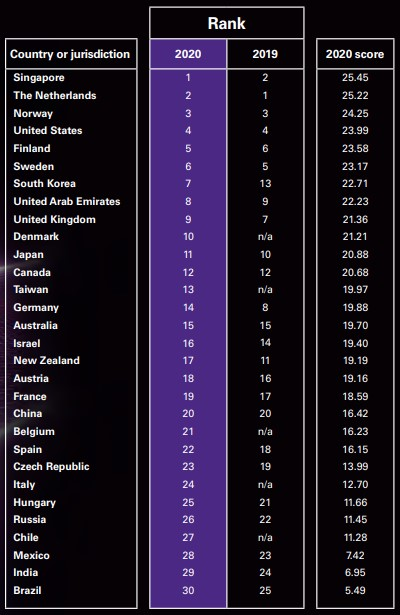
\includegraphics[width=8cm]{Figures/rank.jpg}
\caption{Resultado do relatório 2020 Autonomous Vehicles Readiness Index \cite{KPMG}.}
\label{KPMG}
\end{figure}

Observando o ranking notamos que o Brasil, entre os países estudados, encontra-se na trigésima posição, ficando na última colocação. Dentre os pilares citados e estudados pela KPMG o Brasil apenas não ficou em último lugar na questão de aceitação do consumidor, ficando na vigésima nona posição.
Entre os pontos apresentados o estudo ressalta que o governo brasileira está fazendo muito pouco para encorajar a adoção dos VA, refletindo na última posição do ranking AVRI. Isso apesar do entusiasmo do país por novas tecnologias e serviços, como carona, diz Maurício Endo, chefe de governo da KPMG no Brasil e na América do Sul. “Ainda não vemos nenhuma política pública para criar um caminho para que os VAs comecem a operar nas cidades”.

O programa Rota 2030, lançado em 2018, oferece incentivos para substituir os tipos de motores tradicionais por híbridos ou Veículos Elétricos, embora esse não seja o objetivo principal. Em Outubro de 2019 houve o lançamento de uma pequena frota de carros elétricos Renault Twizy junto com pontos de recarga em Brasília, permitindo que funcionários públicos se desloquem entre prédios do governo de maneira mais econômica e com menos emissões de carbono do que antes.

Por outro lado, o setor privado é mais ativo, embora se concentre nos usos das vias públicas. Em janeiro de 2020, a montadora brasileira de veículos Hitech Electric lançou o que chamou de primeiro VA desenvolvido no país. O e.coTech4 elétrico de dois lugares, que pode atingir velocidades de 50 km/h, está inicialmente disponível apenas para aluguel corporativo em áreas fechadas, como áreas industriais, campus universitários e resorts \cite{KPMG}.

\begin{figure}[H]
\centering
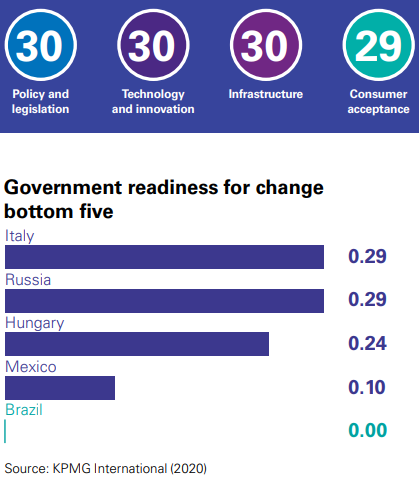
\includegraphics[width=8cm]{Figures/rank30.png}
\caption{Posição do Brasil no relatório \cite{KPMG} 2020.}
\label{rank30}
\end{figure}

Ademais, temos o estudo anual da indústria do Connected Car Innovation Index (CCI) que busca pesquisar empiricamente e comparar o desempenho e a força inovadora de 28 fabricantes globais de automóveis nas áreas de veículos e serviços conectados, bem como sua força de mercado usando vários indicadores. O estudo é baseado no banco de dados de inovação do Centro de Gestão Automotiva (CAM) \cite{CCI}. A partir deste estudo, podemos identificar que o Brasil não encontra-se como uma força inovadora nas áreas de arquitetura veicular, conectividade/infoentretenimento e direção autônoma dos players mais importantes do universo dos carros conectados.


\begin{figure}[H]
\centering
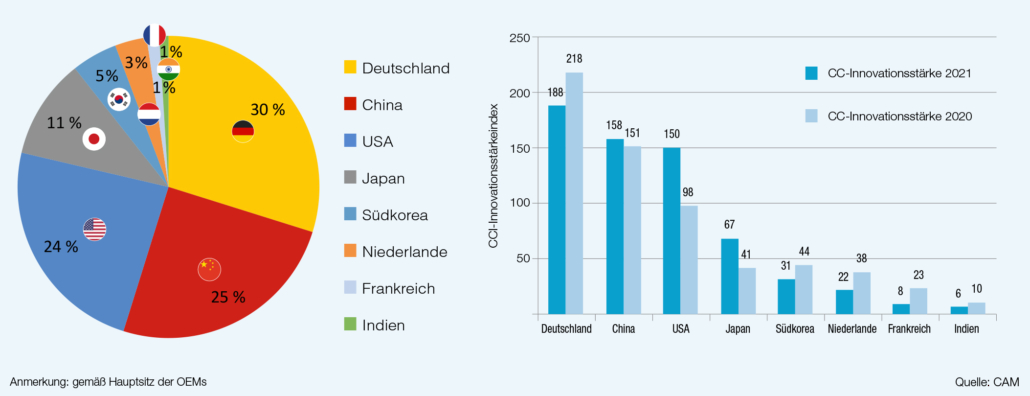
\includegraphics[width=\textwidth]{Figures/CCI.jpg}
\caption{Força inovadora por país  \cite{CCI}.}
\label{forcaCCI}
\end{figure}


Apesar do pouco encorajamento do governo brasileiro quanto a adoração de veículos autônomos, e a baixa aceitação do Brasil comparado com os demais países da lista. Ainda precisamos tratar sobre questões relacionadas à infraestrutura do país para a navegação e operação desses veículos. 
O principal problema que os VAs enfrentarão são os sistemas de sinalização e marcação precários, gerenciamento de tráfego em caso de incidência de tráfego, gerenciamento de estacionamento, proteção de áreas seguras e heterogeneidade do tráfego.

As figuras abaixo mostram uma discussão detalhada dessas principais barreiras e suas implicações no comportamento dos VAs.
\begin{figure}[H]
\centering
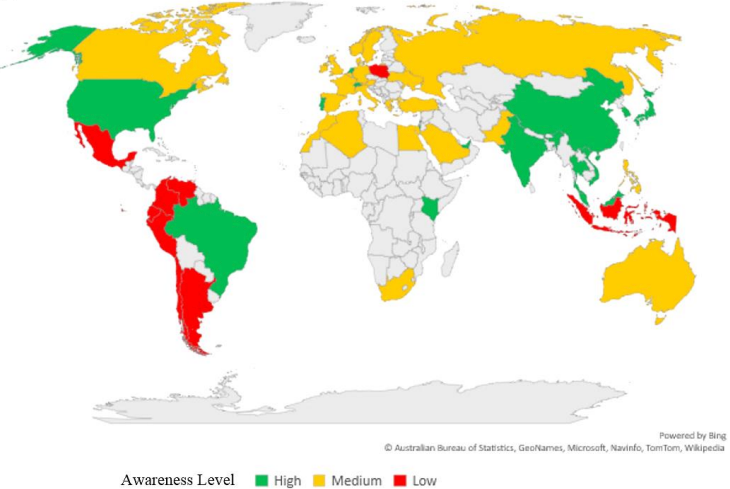
\includegraphics[width=12cm]{Figures/grafik-a.png}
\caption{ Resumo do nível de consciência em diferentes países com diferentes níveis de PIB \cite{mundobrasil}.}
\label{awareness}
\end{figure}
\begin{figure}[H]
\centering
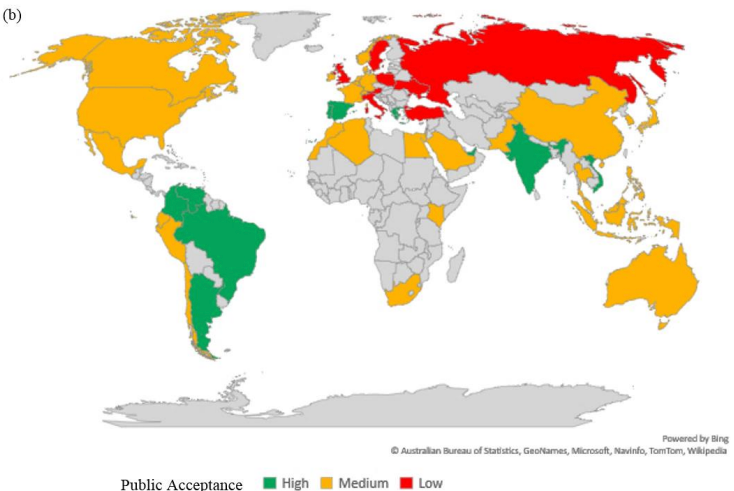
\includegraphics[width=12cm]{Figures/grafik-b.png}
\caption{ Resumo do nível de aceitação pública em relação aos VAs em diferentes países com diferentes níveis de PIB \cite{mundobrasil}.}
\label{public}
\end{figure}

É possível identificar nas figuras \ref{awareness}, \ref{public} que o Brasil encontra-se com um nível alto em consciência e aceitação do público. Para mais detalhes da análise dos principais desafios para a navegação segura de VAs em países em desenvolvimento, \cite{mundobrasil}.


Por fim, como identificado no gráfico \ref{KPMG} Singapura foi o país com maior aproveitamento somando os pilares estudados pelo Autonomous Vehicles Readiness Index 2020, tendo em vista os esforços adicionais que tem feito para encorajar o uso de VAs. Em janeiro de 2019, o governo da cidade-estado publicou seu rascunho de padrões nacionais TR68 para esses veículos, bem como uma estrutura voluntária de governança de IA \cite{KPMG}. A KPMG relata que desde o primeiro relatório publicado os países têm apresentado rápidas e fortes mudanças a caminho da implementação e da ampliação das frotas de veículos autônomos, no desenvolvimento de regularizações e incentivos, além de que a mídia começou a considerar as vantagens e desvantagens dos VAs, empresas testam cada vez mais veículos e os consumidores estão aceitando a ideia de migração para Veículos Autônomos.

\section{Veículos Autônomos e suas perspectivas}

\subsection{Nível de condução autônoma}
	
Na busca de identificar os diferentes tipos de Carro Autônomos, nos deparamos com um cenário ainda em processo de definição. Pois, com os presentes avanços na área de veículos autônomos, surgiu a necessidade, das empresas e dos órgãos de regularização, de classificá-los de alguma forma. Desse modo, A SAE (Society of Automotive Engineers), uma das principais associações globais que busca essa classificação, dividiu os veículos autônomos em seis níveis de funcionalidade, que vão desde nenhum recurso de automação (nível 0) até automação completa, sem a necessidade de um condutor humano, (nível 5). Fazendo uso da terminologia “sistemas de direção autônoma” para se referir a veículos que possuem algum tipo de direção autônoma \cite{SAE}. Nesse cenário, os níveis 1 e 2 incluem alguns recursos, enquanto o nível 3 alcança automação limitada, onde o motorista pode abrir mão do controle do veículo, desde que esteja disponível para intervir.

Abaixo, apresentamos graficamente as diferenças de veículos autônomos e suas respectivas classificações \cite{SAE}:

\begin{figure}[H]
\centering
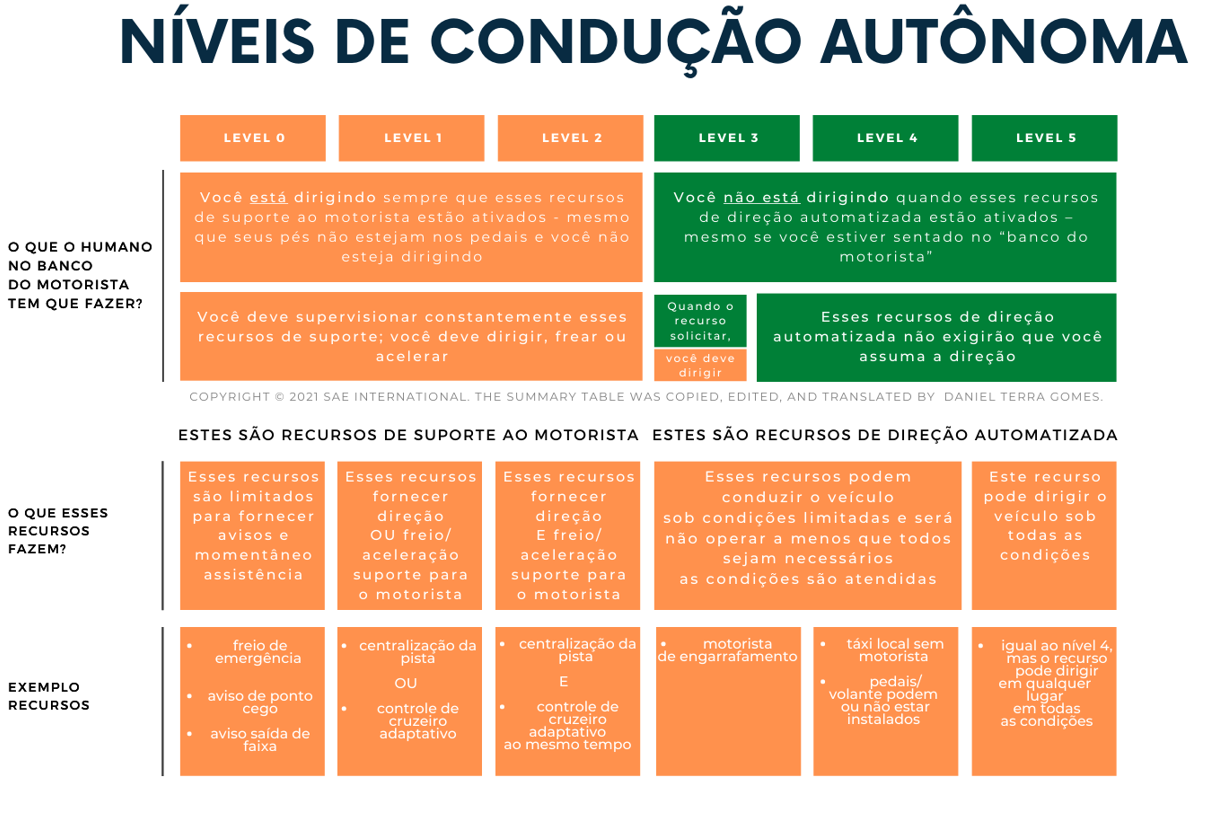
\includegraphics[width=\textwidth]{Figures/IC-Graph1.png}
\caption{Níveis de Automação de condução PT-BR}
\label{Graph_PT}
\end{figure}
\begin{figure}[H]
\centering
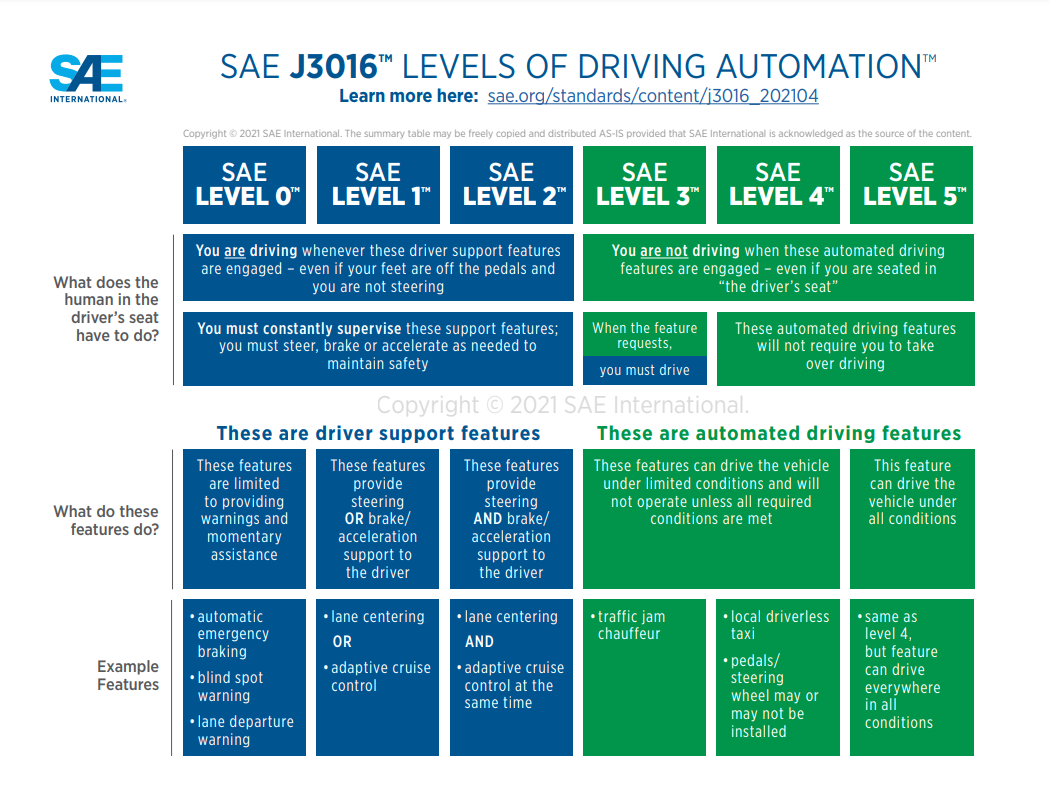
\includegraphics[width=\textwidth]{Figures/IC-GrapEN.png}
\caption{SAE J3016TM levels of driving automation}
\label{Graph_EN}
\end{figure}

Além dessas classificações entre tipos veículos, ainda é possível classificá-los nas seguintes categorias de tipos de automação: Sistema de Assistência Avançada ao Motorista (ADAS) sigla do inglês \textit{advanced driver-assistance system (ADAS)}, ou Condução Automática, Mobilidade Como Serviço (MaaS) sigla do inglês \textit{Mobility as a service (MaaS)}.
Como visto nos gráficos (\ref{Graph_PT} e \ref{Graph_EN}) nos níveis 1, 2 e 3 o condutor precisa estar preparado para caso o sistema precise de algum tipo de ajuda do condutor, esses níveis são vistos como uma espécie de remendo pois funcionam como um remendo para suprir uma demanda que os sistemas autônomos ainda não podem cumprir com maestria \cite{4cenarios_ocidental}. Pois com o avanço da tecnologia o condutor humano torna-se cada vez menos necessário, e como visto no nível 5 (Gráfico \ref{Graph_EN}) é possível a retirada do volante do veículo. 

Na atualidade, empresas líderes do setor de veículos autônomos, como a Tesla, ainda trabalham com nível 2 de direção autônoma referente ao ADAS para veículos vendidos para a população. \cite{4cenarios_ocidental}.
Por outro lado, no início deste ano de 2023, a Mercedes-Benz no seu portal de mídias afirma ser a primeira empresa a alcançar a marca de direção autônoma SAE level 3 para o mercado dos Estados Unidos, sendo o estado de Nevada o primeiro a concordar com as regulamentações para a navegação desses tipos de veículos em seu território. A Mercedes afirma, também, que já em 2024 terá os seus primeiros veículos \textit{DRIVE PILOT}, em portugues “condutor”, disponíveis para o mercado Norte Americano.

“No mundo moderno, o tempo é um dos bens mais preciosos, e devolver o tempo aos nossos clientes é um elemento central em nossa estratégia de construir os carros mais desejados do mundo. O nosso DRIVE PILOT dá um grande passo para o conseguir e coloca-nos na vanguarda da inovação no campo crucialmente importante da condução autónoma. O DRIVE PILOT demonstra mais uma vez que nosso pioneirismo faz parte do nosso DNA. A certificação em Nevada marca o início de seu lançamento internacional e, com ela, o início de uma nova era.” Diz o Markus Schäfer, Membro do Conselho de Administração do Mercedes‑Benz Group AG, Diretor de Tecnologia, responsável por Desenvolvimento e Compras \cite{mercedes3}.

Adicionalmente, algumas empresas, como Waymo e Cruise, atualmente operam serviços de carona com veículos com autonomia de nível 4 nos EUA - isso significa que os carros podem operar sem motorista ao volante sob certas condições, como dentro de uma área de serviço designada, portanto, já mapeadas e entendida pelo algoritmo de controle dos veículos\footnote{Mercedes-Benz wins race to bring Level 3 autonomous cars to US: \url{https://www.freethink.com/hard-tech/drive-pilot}.}.



A seguir forneceremos as definições detalhadas para seis níveis de automação de veículos, variando de nenhuma automação de direção (Nível 0) a automação total de direção (Nível 5), no contexto de veículos a motor, definidos pela SAE \cite{SAE}:

\begin{enumerate}
 \item \textbf{Nível 0} – Sem automação de condução: Não existe nenhum tipo de auxílio ao motorista e nenhuma presença/atuação de tecnologia de condução autônoma, ou assistência.

\item \textbf{Nível 1} - Assistência ao Motorista: No nível 1, o motorista é assistido apenas em relação à velocidade do veículo, um exemplo prático seria o piloto automático, que mantém a velocidade do veículo constante de acordo com o gosto do motorista. Neste caso, o condutor deve continuar a frear, acelerar e direcionar o veículo. Um segundo exemplo seria: o recurso de assistência ao estacionamento, executa automaticamente as ações de controle de movimento do veículo necessárias para estacionar um veículo, enquanto o motorista executa as ações de controle de movimento do veículo longitudinal e supervisiona o recurso de estacionamento.

\item \textbf{Nível 2} - Automação de Condução parcial: Nesta fase, o veículo já é capaz de realizar ações de forma autônoma, como frear, acelerar e parar o veículo em uma direção, como é o caso da tecnologia chamada ACC (Adaptive Cruise Control). No nível 2, o condutor continua a ser responsável pela condução e exige que o condutor esteja atento à condução e retome a condução em situações de perigo. Um exemplo prático seria, como visto: o recurso de assistência ao estacionamento, mas dessa vez, executa automaticamente as ações de controle de movimento lateral e longitudinal do veículo, necessárias para estacionar um veículo sob a supervisão do motorista.

\item \textbf{Nível 3} - Automação Condicional de Condução: Consiste em veículos que são capazes de se mover de forma independente, tanto na direção, aceleração e frenagem. Neste nível de condução, o condutor pode realizar outras atividades enquanto o carro segue autonomamente a sua rota, mas por vezes é acionado para assumir a condução por um curto período de tempo ou para assumir o controlo total em situações de risco. Nesse cenário, um \textit{automated driving system} (ADS)  é capaz de continuar a executar o \textit{dynamic driving task} (DDT) por pelo menos vários segundos após fornecer ao usuário pronto para \textit{fallback}; uma solicitação para intervir. Espera-se então que o usuário pronto para o \textit{fallback} do DDT retome a operação manual do veículo ou alcance uma condição de risco mínimo se ele/ela/elu determinar que é necessário.

\item \textbf{Nível 4} - Alta Automação de Condução: O veículo controla todas as tarefas 
que antes eram do condutor, sem necessidade da atenção do mesmo. Desse modo, o veículo fica em cargo de executar todo o DDT em uma localidade, ao sofrer uma falha de sistema relevante para o desempenho do DDT. Em resposta, o \textit{ADS-dedicated vehicle} (ADS-DV) realiza o \textit{fallback} do DDT ligando os piscas de emergência, manobrando o veículo para o acostamento e estacionando-o, antes de chamar automaticamente a assistência de emergência. Nesse  nível, o ADS é capaz de atingir automaticamente uma condição de risco mínimo quando necessário.

\item \textbf{Nível 5} - Automação de Condução completa: permite que o veículo elimine a necessidade de um motorista humano, com todos os controles e tarefas de direção realizados por um sistema autônomo. O desempenho do veículo é sustentado, incondicionalmente, por um ADS responsável por todo o DDT e \textit{fallback} do DDT sem qualquer expectativa de que um usuário precise intervir.

\end{enumerate}

\subsection{Condução Autônoma e mercado tecnológico}

A inserção da Condução Autônoma no mercado dependerá da demanda de viagens por veículos, da infraestrutura de transporte, do grau de automação desses veículos, da taxa na qual os veículos autônomos são introduzidos no mercado, e da confiança da sociedade com essa categoria de transporte. 

Como visto, no gráfico (Gráfico \ref{Graph_EN}) os níveis de automação de 0 a 3 exigirão a presença de um motorista no veículo. O nível 4 a 5, não fazem a exigência de ter a presença de um motorista humano na tarefa de monitorar constantemente o ambiente de direção. 
Abrindo categorias inteiramente novas de viagens, com a não necessidade de um motorista humano para a realização do transporte da população \cite{notif}.

Nessa realidade, onde não há mais a necessidade de um condutor humano para o veículo (Carro de Passeio). Haverá a possibilidade das pessoas se engajarem em outras atividades, pois agora a sua atenção não precisa está direcionada em conduzir ou assistir o veículo para alcançar o destino programado. 

\begin{figure}[H]
\centering
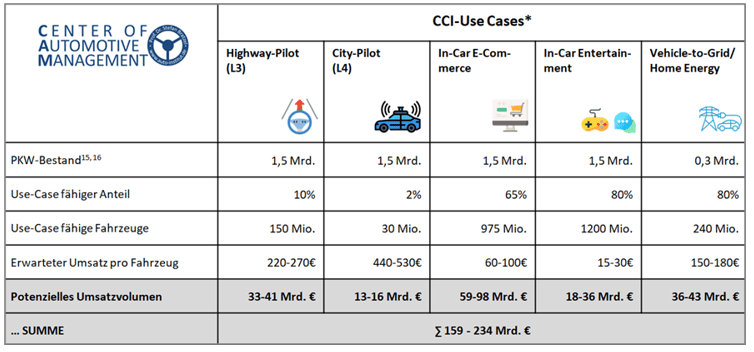
\includegraphics[width=\textwidth]{Figures/grafik-2.png}
\caption{ Lista potencial de mercado de Serviços conectados em todo o mundo em 2030, por casos de uso \cite{CAM}.}
\label{conectados}
\end{figure}


Mas isso ainda é algo para 2029 \cite{elpais}, data em que El País dá a sua previsão. Por outro lado, atualmente, a direção autônoma ainda funciona como um assistente para o condutor; os assistindo em trocas de faixas, estacionamento, controle de velocidade, entre outras coisas. 

Nesse sentido, trabalham as marcas de luxo onde essas tecnologias são mais comuns, devido ao alto custo de desenvolvimento. Desse modo, os consumidores podem, já hoje, ter acesso a veículos autónomos. Entretanto, esses veículos são definidos como semi autônomos classificados como nível 2 (Gráfico \ref{Graph_EN}) SAE. As principais marcas estadunidenses automotivas que trabalham, hoje, como essa tecnologia são:  Tesla, Cadillac, Audi, BMW, Mercedes-Benz, Jaguar, Land Rover \cite{caio}. 
Dessas marcas a que representa maiores avanços, segundo as pesquisas, é a Mercedes-Benz, sendo  a primeira das marcas a começar a sua produção já em 2024 de veículos comerciais com nível 3 SAE \cite{mercedes3}.
No outro espectro, há os veículos de carona que têm como essência ser carros autônomos que operam no nível 4 e 5 SAE, comumente conhecidos como Táxi Robô. Na atualidade, apenas algumas empresas trabalham com essa categoria de veículo. Esses carros, hoje, se situam no nível 3 - 4 de autonomia, operando apenas em rotas já cadastradas em seus bancos de dados, portanto em locais já conhecidos e sem muitas chances de situações extremas, fora das suas bases de dados. 

As principais empresas que trabalham no desenvolvimento dessa categoria de veículo são, por exemplo:

\begin{enumerate}

   \item \textbf{Waymo (Alphabet):}
         Trabalhando com veículos no nível 4 SAE. Entretanto, fazendo uso de seres humanos de maneira remota para dar assistência aos seus veículos quando necessário \cite{waymo}. Atualmente, a Waymo, subsidiária da Alphabet, possui as mais altas competências, incluindo a mais extensa experiência em testes do mercado\cite{CAM};
   \item \textbf{Zoox (Amazon):}
         Sua frota de veículos de carona operam no nível 3 \cite{zoox};
   \item \textbf{Uber:}
         Atualmente, seus veículos trabalham em nível 3 e estão a realizar testes em nível 4 SAE. Cujo é o objetivo da empresa pois a indústria automotiva define esse nível como "atenção desligada” \cite{uber};
   \item \textbf{Mobileye (Intel):}
         A frota de veículos hoje opera em nível equivalente ao 4 SAE. A empresa busca a sua própria taxonomia de seus veículos \cite{mobileye}, \cite{mobileye1}.
\end{enumerate}

Lista completa das empresas no domínio dos “sistemas de condução autónoma”:


\begin{figure}[H]
\centering
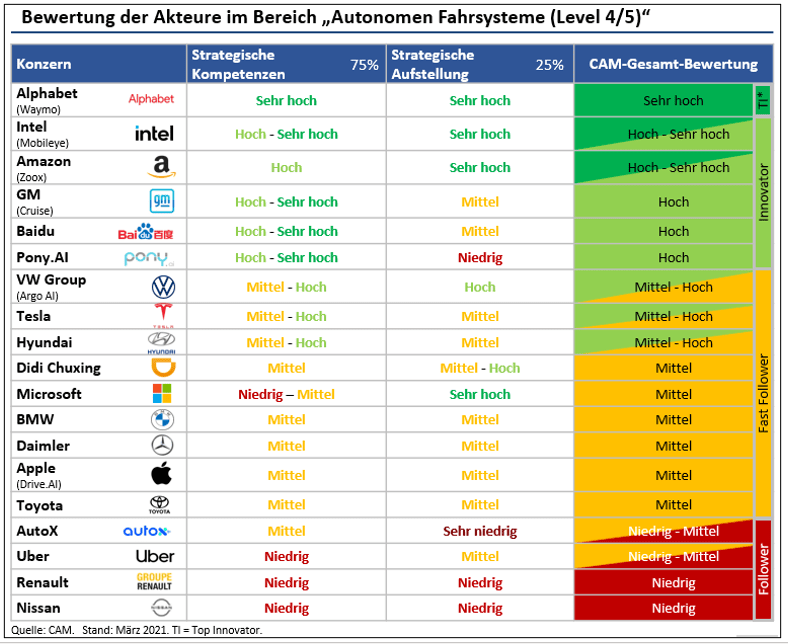
\includegraphics[width=16cm]{Figures/grafik.png}
\caption{ Listas das empresas no domínio dos “sistemas de condução autónoma” (Nível 4/5) 2021 \cite{CAM}.}
\label{figura_companies}
\end{figure}

A partir dessa listagem, podemos ter uma melhor compreensão de como se encontra o cenário das empresas que hoje trabalham com veículos que possuem algum tipo de recurso autônomo, referente ao SAE. Listagem oriunda da (CAM) \textit{The Center of Automotive Management}; fornece com base em métodos científicos e bancos de dados abrangentes, orientações confiáveis sobre o universo automobilístico.

\vspace {1cm}

Na perspectiva de crescimento econômico, e investimento no setor automobilístico em relação a veículos autônomos. O CEO da GM, Mary Barra, diz estar investindo agressivamente no mercado, com um plano de investimento de US \$35 bilhões para veículos movidos a bateria e autônomos \cite{gm}.



\section{Tecnologias Essenciais para a Direção Autônoma}


\subsection{TO DO}



\subsection{DELETE}
Nesse primeiro subprojeto buscamos estruturar uma definição para a ciência de dados a partir dos artigos estudados. 

\subsubsection{O que é Ciência de Dados?}
\cite{BATON} define a ciência de dados como o campo multidisciplinar que busca novas ideias a partir de dados do mundo real através da aplicação estruturada de técnicas primariamente estatísticas e computacionais. 
O artigo também afirma que na literatura ainda há considerável debate quanto aos contornos desse campo, porém, os especialistas tendem a concordar que a necessidade de integrar diversas disciplinas, aliada aos desafios de criar uma infraestrutura analítica robusta, introduziram um conjunto único de desafios que são melhor enfrentados por profissionais chamados "cientistas de dados". Ao que \cite{DONOHO} acrescenta:
\begin{quote}
"Ciência de Dados" é o melhor campo para acomodar pesquisa de grande impacto que seria difícil de classificar de outro modo, como por exemplo Tukey 1977 EDA e o trabalho de Wickham em Tidy Data e Grammar of Graphics.
\end{quote}

Essa nova ciência, conclamada em 1962 por John Tukey, foi recebida com timidez e controvérsia entre os estatísticos. Mas, meio século depois, com a popularização de linguagens e ambientes de programação quantitativos como o R\cite{ihaka1996r},  ela se tornou auto-evidente. Isto porque o que antes era uma descrição em prosa de uma análise, agora poderia ser precisamente descrito em um \textsc{script} com alto nível de abstração. Esses chamados \\textit{workflows} podem ser compartilhados, reexecutados com outros dados, facilmente modificados e quantificados. Logo, se tornaram evidentes objetos de pesquisa, \cite{DONOHO}.

Ambos os artigos \cite{BATON,DONOHO} observaram na literatura a precisão da profecia de Tukey, especialmente em sua afirmativa sobre a Ciência de Dados ser uma disciplina orientada pela prática. Ou seja, seu sucesso deriva do valor gerado ao resolver problemas do mundo real, maximizar resultados, e a sua efetividade em gerar valor. 

\subsubsection{Processos que constituem a Ciência de dados}
Outra dimensão ressaltada por Tukey e observada por \cite{DONOHO} especialmente nas ideias de John Chambers\cite{CHAMBERS} and Bill Cleveland\cite{cleveland2001data} é a ciência que se forma no entorno do "aprender com dados do mundo real" e tudo que esse processo engloba. Especialmente a possibilidade da Ciência de Dados construir e oferecer ferramental que possibilite o avanço de todas as outras ciências, ao aprimorar todo o processo de transformar dados em informação, desde ferramentas de processamento computacional, até bases epistemológicas desse processo. 

\cite{DONOHO} chama essa disciplina expandida de \\textit{Greater Data Science (GDS)}, e a divide em seis sub-áreas:
\begin{enumerate}
\item Data Gathering, Preparation, and Exploration
\item Data Representation and Transformation
\item Computing with Data
\item Data Modeling 
\item Data Visualization and Presentation
\item Science about Data Science

\end{enumerate}
Já \cite{BATON} traz uma abordagem observacional, processando o que já está registrado na literatura com pesquisas de mercado. O artigo sintetiza o Modelo de Trabalho ou \emph{Data Work Model}, constituído de quatro processos de alta ordem, divididos em 14 subprocessos da seguinte forma:
\begin{itemize}
\item \textbf{Preparation}: Defining Needs, Data Gathering, Data Creation, Profiling, and Data Wrangling
\item \textbf{Analysis}: Experimentation, Exploration, Modeling, Verification, and Interpretation.
\item \textbf{Deployment}: Monitoring and Refinement
\item \textbf{Communication}: Dissemination and Documentation
\end{itemize}

O artigo também identifica mais dois processos de alta ordem emergindo:
\begin{itemize}
\item \textbf{Pedagogy} 
\item \textbf{Collaboration}
\end{itemize}

Podemos observar que ambas as definições são compatíveis e adequadas à sua proposta: a GDS \cite{DONOHO} como orientação teórica de pesquisa e organização da literatura, enquanto o Data Work Model \cite{BATON} oferece uma excelente estrutura para abordar um projeto de dados. 

\subsection{Definição de problemas de dados}
\subsubsection{Principais conceitos}\label{principais.conceitos}
 O livro \cite{DATAPYTHON} ressalta a importância fundamental de se entender o "problema do negócio" e circunscreve-lo em uma definição matemática. O que muitas vezes significa ter um papel fundamental na definição do "que será feito e como será feito". Portanto, a ciência de dados requer um diálogo imprescindível entre o cientista e pessoas especializadas na área do "negócio".
 
Nesse sentido, segundo o modelo \cite{BATON}, a definição do problema de dados é o processo de traduzir objetivos analíticos, geralmente definidos pelas parte interessadas, em um conjunto de requerimentos viáveis. Dentre tais requerimentos estão:
\begin{itemize}
\item Dados necessários
\item Planos para analisá-los
\item Definir quais serão as entregas, como por exemplo: relatórios, modelos e infraestrutura computacional. 
\end{itemize}

\subsubsection{Titanic}

No projeto Titanic, e nas competições Kaggle em geral, já temos o "problema de negócio" definido. Nesse caso, nosso problema é determinar a partir dos seus dados, quais passageiros sobreviveriam ao trágico acidente, tendo em vista, especialmente um olhar crítico para os resultados, analisando quais foram as características dos passageiros que aumentaram suas chances de sobrevivência.

A partir desse problema devemos pensar em quais dados precisamos obter para aborda-lo. Nesse caso, precisamos de uma amostra com os dados de diversos passageiros e o seu destino. Podemos utilizar tal amostra para treinar um modelo preditivo que possa receber outro conjunto análogo apenas com as informações e predizer o destino de cada um. Dessa forma, no processo de construção desse modelo esperamos compreender quais foram os fatores que mais contribuíram para o desfecho de cada pessoa à bordo. 

Já temos nessa etapa da definição do problema, conceitos iniciais de \\textit{Aprendizado de Máquina}. Isto porque temos uma variável a ser predita, também chamada de variável alvo (\textbf{target}), variável resposta ou \textbf{y}. 
Para predize-la, temos um conjunto de \textbf{features}, isto é, as características de cada passageiro em nosso conjunto de dados, também chamado de \\textit{DataFrame ou DataSet}. A partir das \emph{features}, geramos um conjunto de variáveis \textbf{X} para prever nossa variável \textbf{y}. 
Dessa forma, precisamos de um \emph{dataset} com \emph{features} e variável alvo. 
Estes dados de treino são inseridos em um modelo que tentará modelar matematicamente as relações de X para y, de modo que posteriormente para qualquer outro conjunto análogo a X, o modelo possa prever um valor de y. 

Assim, sabemos que devemos construir um modelo preditivo de classificação, que para cada conjunto de dados $X_i$ de um passageiro \emph{i}, ele possa gerar um $y_i$ de valor zero ou um, representando a sua sobrevivência. Também sabemos que se faz necessário, portanto, obtermos um \emph{dataset} com X e y para treinarmos nosso modelo. O que também já nos aponta para o uso da biblioteca Pandas para estruturar esse X além do uso da biblioteca \emph{Scikit Learn} para criar, treinar e utilizar um modelo de Aprendizado de Máquina em português.

\subsection{Obtenção de Dados}
\subsubsection{Conceitos principais}
Uma vez definidos os requerimentos, o passo seguinte de acordo com o modelo \cite{BATON}, é a obtenção de dados. Para tanto, o modelo ressalta três possibilidades:
\begin{itemize}
\item Identificar o conjunto de dados adequado dentre vários candidatos. 
\item Gerar novos dados a partir da integração e transformação de dois ou mais conjuntos existentes. 
\item Desenvolver critérios e mecanismos para coletar dados que ainda não existem. 
\end{itemize}
 
Tanto a primeira, quanto a segunda situação se referem aos casos nos quais o "cliente" do serviço de dados já dispõem de um banco de dados estruturado. Nesse caso, normalmente, a obtenção envolve escrever uma \emph{query} na linguagem SQL.  
 Do contrário, quando o cliente dispõem dos dados porém em formato inadequado,  é necessário primariamente adequá-los ao primeiro caso, o que normalmente também envolverá a linguagem SQL, provavelmente \emph{scritps} e possivelmente certa organização manual de dados.  

 No terceiro caso, há uma variedade maior de possibilidades, desde a realização de pesquisa como questionários, até a criação de \emph{scritps} para capturar da internet as informações relevantes, processo que chamamos de \emph{Webscrapping}\cite{mitchell2018web}. 
  
O livro \cite{DATAPYTHON} também ressalta a importância da documentação do conjunto de dados obtidos. Nela devem estar as principais informações sobre o \emph{dataset}, tais como a explicação de suas colunas e seus conteúdos, definições de termos, seu contexto, dentre outras. 

 \subsubsection{SQL}
Conforme mencionamos na metodologia, a linguagem SQL não foi necessária no projeto Titanic, entretanto muitos autores como \cite{SCRATCH,DATAPYTHON} ressaltam a sua importância, especialmente no ferramental de um cientista de dados. \cite{debarros2022practical} a define da seguinte maneira:
\begin{quote}
    SQL é uma linguagem de programação amplamente utilizada que permite definir e consultar bancos de dados. Seja você um analista de marketing, um jornalista ou um pesquisador mapeando neurônios no cérebro de uma mosca, você se beneficiará do uso do SQL para gerenciar objetos de banco de dados, bem como criar, modificar, explorar e resumir dados. 
\end{quote}

Nesse sentido, elencamos recursos para aprender essa habilidade que esperamos nos aprofundar nos próximos trabalhos. Identificamos os livros \cite{debarros2022practical,Silberschatz2019DBS} como as referências interessantes. Além deles, acreditamos que a forma mais eficiente de se aprender uma habilidade prática é por meio da prática direcionada, nesse sentido, os seguintes sites se mostraram os mais eficientes em apresentar exercícios práticos: 
\begin{itemize}
\item \href{https://sqlbolt.com/}{SQLbolt} \footnote{sqlbolt.com/}
\item \href{https://www.hackerrank.com/domains/sql}{Hacker Rank}\footnote{www.hackerrank.com/domains/sql}
\item \href{https://pgexercises.com/}{PostgreSQL Exercises}\footnote{pgexercises.com}
\end{itemize}
 
 \subsubsection{Titanic}
À partir da definição do problema, buscamos obter os dados disponíveis ou criá-los. No caso de nosso projeto Titanic, como em todas as competições Kaggle, os dados são disponibilizados pela plataforma e podem ser obtidos conforme descrito na metodologia. Temos, portanto, os \emph{DataFrames}  para o treinamento e validação do modelo, predição e submissão à plataforma Kaggle e exemplo de submissão derivados dos arquivos \emph{train.csv, test.csv, e gender\_submission.csv} respectivamente apresentados nas Figuras \ref{df.csv}, \ref{test.csv} e \ref{gender.submission.csv} respectivas. 
\begin{figure}[H]
\centering
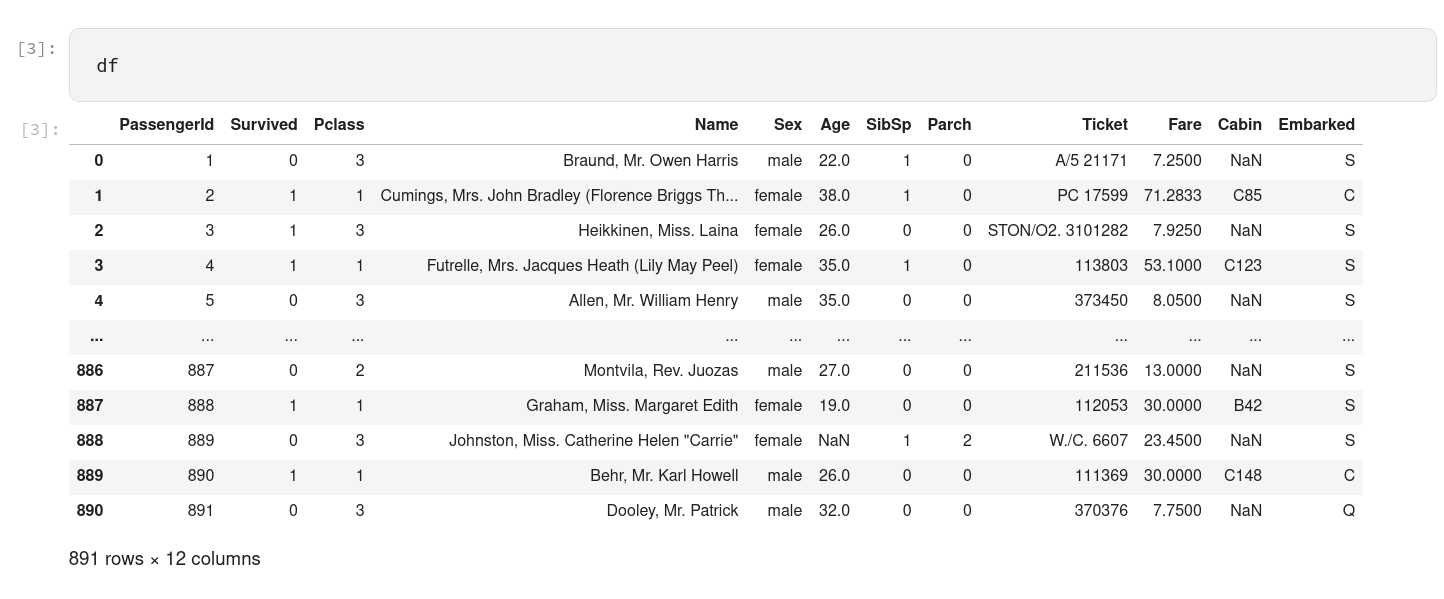
\includegraphics[width=\textwidth]{Figures/df.png}
\caption{\emph{DataFrame} NÍVEIS DE AUTOMAÇÃO DE CONDUÇÃO PT}
\label{df.csv}
\end{figure}
\begin{figure}[H]
\centering
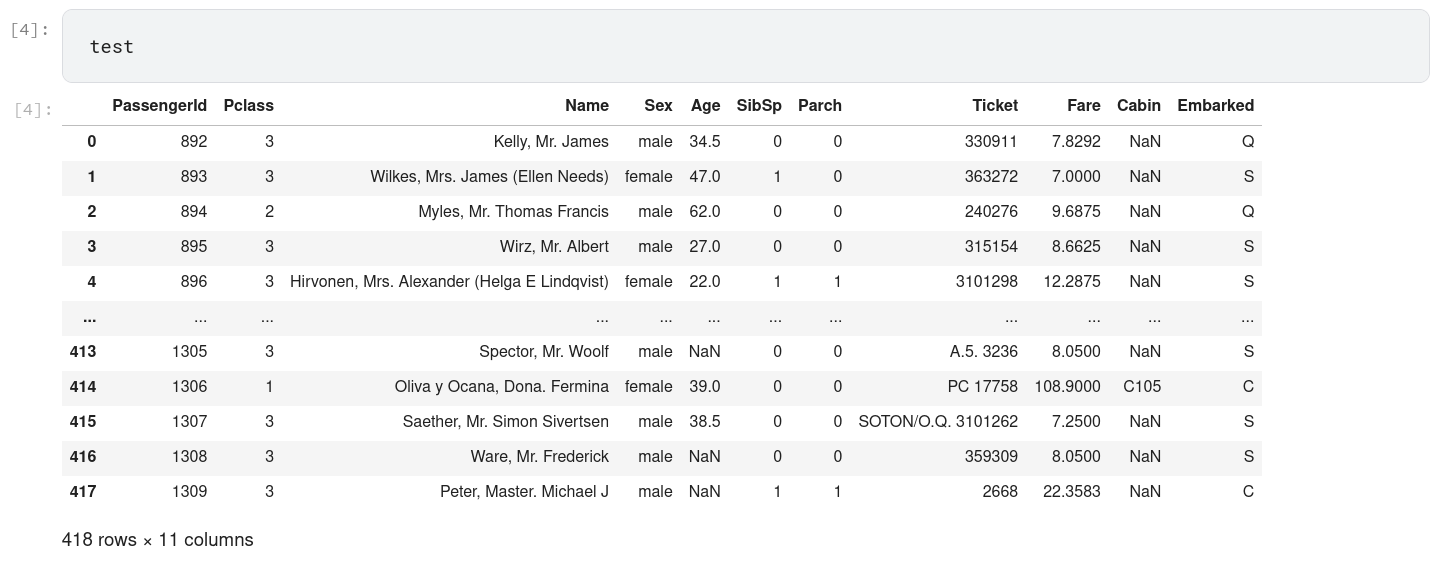
\includegraphics[width=\textwidth]{Figures/test.png}
\caption{SAE J3016TM LEVELS OF DRIVING AUTOMATIONT}
\label{test.csv}
\end{figure}
\begin{figure}[H]
\centering
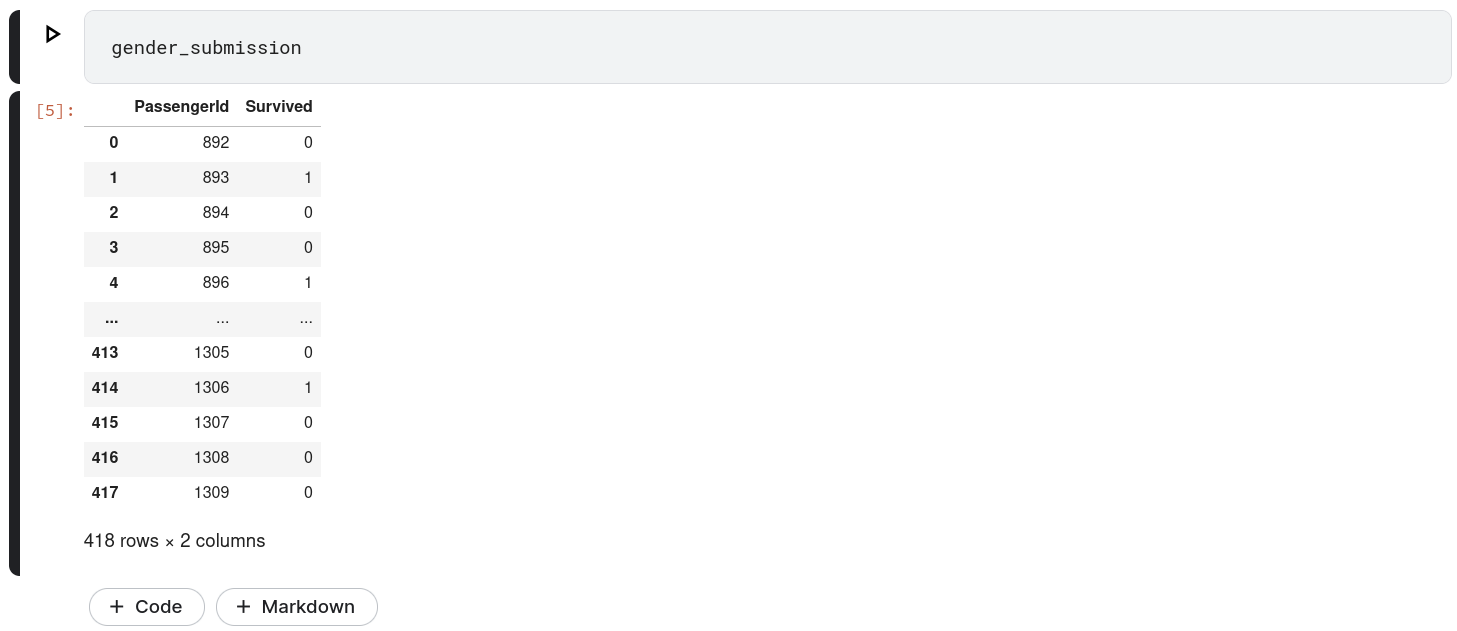
\includegraphics[width=\textwidth]{Figures/gender_submission.png}
\caption{\emph{DataFrame} gender\_submission.csv submetido à plataforma Kaggle}
\label{gender.submission.csv}
\end{figure}

\begin{itemize}
\item \emph{train.csv}:  uma tabela com 891 linhas e 12 colunas, respectivamente representando cada passageiro, e suas \emph{features}, inclusive se ele sobreviveu. Exatamente o \emph{dataset} descrito em nosso requerimento, portanto será o nosso principal \emph{DataFrame} de trabalho, que iremos analisar, transformar e utilizar para treinar nosso modelo preditivo.  
\item \emph{test.csv}: muito semelhante ao arquivo anterior, contem outros 418 passageiros, mas dessa vez apenas 11 colunas. Isto porque a coluna "\textsc{survived}" está ausente, exatamente a coluna que nosso modelo se propõe a preencher. Este, é o conjunto de dados cuja resposta será utilizada na avaliação automática que o kaggle faz em nosso modelo. 
\item \emph{gender\_submission.csv}: é um exemplo de submissão a competição kaggle, ela contém as mesmas 418 linhas e a mesma coluna "\textsc{PassengerId}" que o arquivo \emph{test.csv} contém, acrescida da coluna "\textsc{Survived}", nesse caso, preenchida a título de exemplo de modo que todas as passageiras sobreviveram e todos os passageiros morreram. Esse é um exemplo do arquivo que será submetido a competição e utilizado para avaliar nossa solução para o problema. 
\end{itemize}

\subsection{Data Analysis}
\subsubsection{Conceitos principais}
\cite{BATON} aponta que esse processo, denominado de Data Analysis pelo livro \cite{DATAPYTHON}, também pode ser encontrado com outros nomes na literatura como "pré-processamento", "tidying", "limpeza", "wrangling", "Exploratory Data Analysis (EDA)" ou ainda "Data Understanding". 
Nesse sentido, as autoras defendem dividi-lo entre "Profiling" e "Data Wrangling" e agrupa-los junto aos passos anteriores, de modo a constituir o macro processo de "Preparation". 

Assim, de acordo com o modelo apresentado, temos as seguintes definições:
\begin{itemize}
\item \textbf{Profiling}: é o processo de avaliar atributos dos dados para entender a distribuição de seus valores, identificar valores faltantes e examinar a sua associação à outros atributos. Bem como compreender os dados e seu conteúdo. 
\item \textbf{Data Wrangling}: processo de utilizar o que foi aprendido no Profiling para conformar e transformar os dados de modo a adequá-los para os próximos passos. 
\end{itemize}

Nesse sentido, dentro do ecossistema Python, a biblioteca Pandas é a ferramenta absoluta para manipulação de tabelas, aliada a NumPy, que traz um robusto repertório de implementações matemáticas e aplicações de álgebra linear.\cite{PRINCIPLES}

\subsubsection{Técnicas}
Segundo \cite{BATON,DONOHO,DATAPYTHON} Essa etapa é sabidamente a mais dispendiosa de um projeto de dados. Devido principalmente ao tempo necessário e dificuldade de automatizar. Dessa forma, é também uma das etapas mais difíceis de se ensinar justamente em função da intervenção humana e seu processo quase artesanal para compreender adequar os dados. 

Dessa forma, segundo \cite{DATAPYTHON}, devemos analisar os dados tanto diretamente quanto por meio de sumários gráficos e numéricos, mas principalmente analisar criticamente se nossos achados fazem sentido, e se estão de acordo com a documentação do dataset. Nesse sentido compilamos a seguinte lista de perguntas para nortear o processo de \emph{Profiling}:
\begin{enumerate}
\item Quantas colunas? (podem ser features, variável resposta, ou metadados)
\item Quantas linhas? (checar se cada linha é uma amostra)
\item Quais são os tipos de features? Quais são categóricas e quais são numéricas? 
\item Como são esses dados? (em numéricas podemos examinar range de valores, ou frequência de diferentes classes em categóricas por exemplo)
\item Temos valores faltantes? 
\end{enumerate}
Se o dataset for pequeno o bastante podemos examinar individualmente cada feature. Já quando o dataset tem centenas de features devemos explorar técnicas de redução de dimensionalidade, que condensam informação em um número menor de features derivadas ou métodos de feature selection que podem auxiliar a encontrar features importantes dentre muitas candidatas. Nesse sentido, \cite{DATAPYTHON} afirma:
\begin{quote}
    "Tempo dedicado analisando critica e detalhadamente se um dataset cumpre seu propósito é um tempo bem gasto." 
\end{quote}

\subsubsection{Titanic}
No projeto Titanic, portanto, iniciamos o \emph{Profilling} do nosso arquivo principal \emph{train.csv}, por meio da variável "\textsc{df}" orientados pela lista de perguntas que construímos.

Como podemos observar na Figura \ref{df.info}, temos 12 colunas ou \emph{features} e 891 linhas ou \emph{dados}. Também logo observamos que as colunas \textsc{Age, Cabin} e \textsc{Embarked} tem dados faltantes. As outras 9 \emph{features} estão totalmente preenchidas. 
Observamos por meio do atributo \emph{Dtype} que as colunas \textsc{Name, Sex, Ticket, Cabin} e \textsc{Embarked} são variáveis categóricas (definidas como tipo \emph{object}), enquanto as outras são numéricas. Podemos confirmar tal fato observando os conteúdos da tabela de treinamento mostrada na Figura \ref{df.csv} onde podemos ver as primeiras e últimas entradas desta tabela de treinamento.
\begin{figure}[H]
\centering
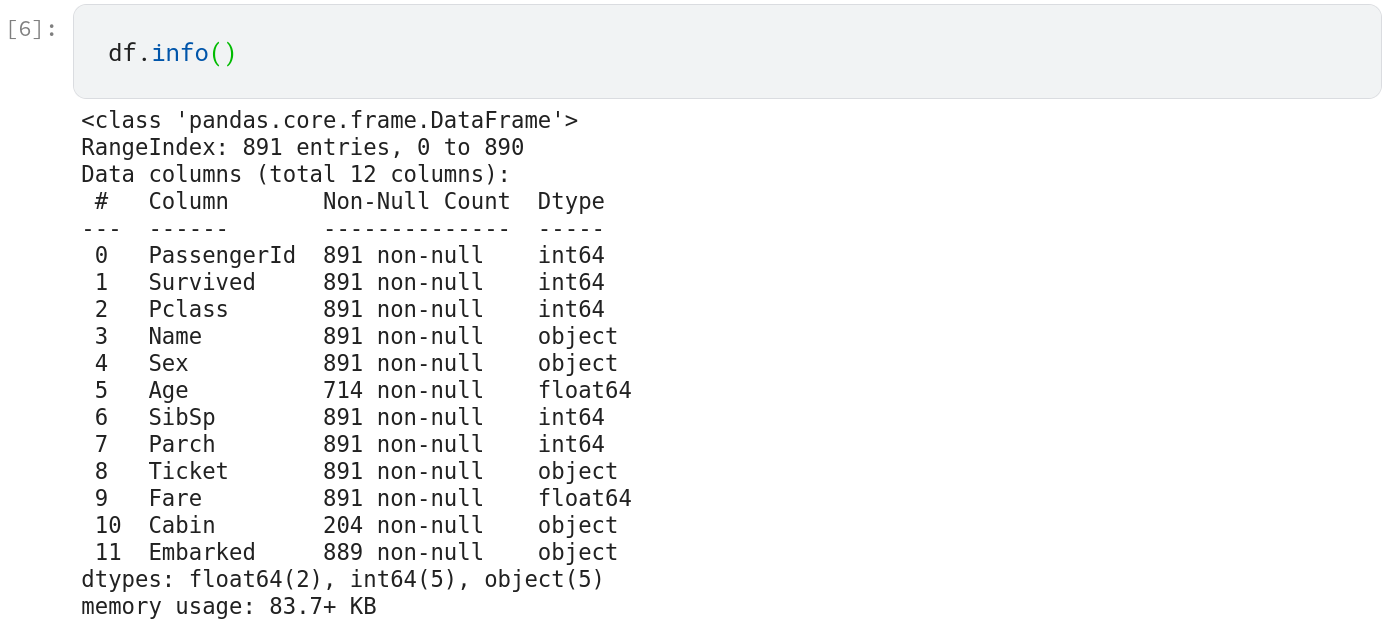
\includegraphics[width=\textwidth]{Figures/df.info().png}
\caption{\label{df.info}Informação sobre a tabela de treinamento, usando o comando \textsc{df.info()}}
\end{figure}

Logo em seguida observamos a tabela \textsc{df} e estudamos a documentação do \emph{DataSet} para compreender cada uma das 12 colunas/features. Na sequência apresenta-se o significado de cada uma destas colunas no Projeto Titanic:
\begin{itemize}
\item \textsc{PassengerId}: o número que representa cada passageiro. 
\item \textsc{Survived}: 0 ou 1, para representar se determinado passageiro sobreviveu.
\item \textsc{Pclass}: classe do ticket do passageiro. Equivalente a classe economica 1-alta;2-media;3-baixa
\item \textsc{Name}: nome do passageiro com sobrenome e pronome de tratamento. 
\item \textsc{Sex}: masculino ou feminino. 
\item \textsc{Age}: idade em anos, em bebês abaixo de 1 ano é uma fração estimada. 
\item \textsc{SibSp}: \# irmãos e cônjuges a bordo.
\item \textsc{Parch}: \# paretens e filhos a bordo. 
\item \textsc{Ticket}: número do ticket
\item \textsc{Fare}: Tarifa paga pelo passageiro. 
\item \textsc{Cabin}: Número da cabine. 
\item \textsc{Embarked}: Porto de embarque. C = Cherbourg, Q = Queenstown, S = Southampton
\end{itemize}

Na sequência, analisamos suas principais métricas (média, desvio padrão, quartis). Na Figura \ref{df.describe} se apresenta o resultado da execução do comando \textsc{df.describe()}.
\begin{figure}[H]
\centering
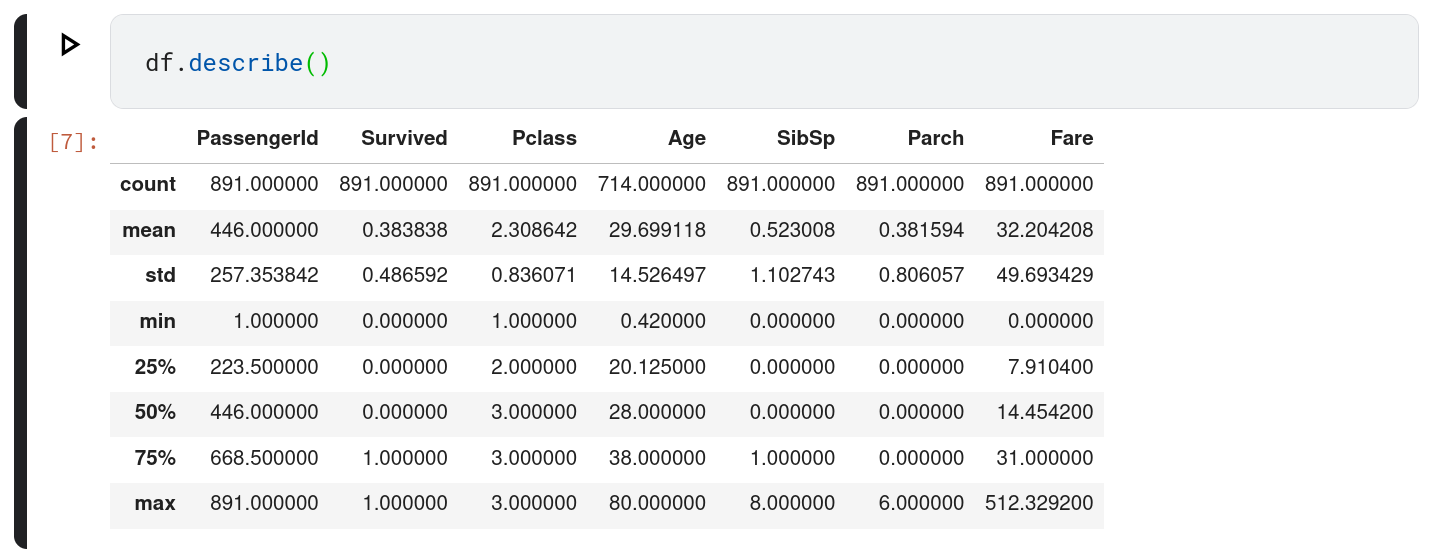
\includegraphics[width=\textwidth]{Figures/df.describe().png}
\caption{\label{df.describe}Estatística descritiva dos dados do treinamento.}
\end{figure}

A partir dessas observações podemos desenvolver as seguintes suposições:
\begin{itemize}
\item \textsc{PassengerID} pode ser desconsiderada, uma vez que é apenas um artefato computacional para denominar as colunas.
\item \textsc{Name} a princípio também será desconsiderado, uma vez que é pouco provável que tenha uma relação direta com a sobrevivência portanto a complexidade de quantificá-la não parece valer. 
\item \textsc{Sex} pode ser convertida em 0 e 1. 
\item \textsc{Age} tem um número considerável de linhas com dados faltantes, poderíamos excluí-la, porem faria sentido a idade ter alguma relação com a sobrevivência, nesse caso iremos lidar com os valores faltantes. Também podemos criar uma \emph{Feature} com intervalos de idade. 
\item \textsc{SibSp} e \textsc{Parch} podem ser combinados em uma terceira \emph{feature} que combina os familiares à bordo, seria interessante saber se deveríamos somar ou multiplicar esses números. 
\item \textsc{Ticket} também pode ser, a princípio, desconsiderado, uma vez que não temos na documentação a explicação de seu código alfa numérico, e assim como \textsc{Name}, essa \emph{feature} não parece ter direta relação com a sobrevivência. 
\item  \textsc{Fare}, parece bem promissora, uma vez que não apresenta dados faltantes, já é numérica, e parece ter uma relação clara com a sobrevivência.  
\item \textsc{Cabin}, assim como \textsc{ticket}, não temos uma tradução numérica, poderíamos construir uma \emph{Feature} como a contagem de cabines, entretanto temos muitos valores faltantes, portanto, é provável que desconsidera-la seja a melhor opção. 
\item \textsc{Embarked}, pode ter alguma relação coma sobrevivência, provavelmente a trataremos. 
\end{itemize}

Podemos utilizar a pivotagem pra nos indicar a importância relativa de nossas \emph{features} numéricas, ou seja, agrupar cada uma delas de acordo com a sobrevivência por meio de suas médias. Assim teremos para cada coluna o seu valor médio entre os sobreviventes e entre os não sobreviventes, desse modo, variáveis que foram importantes como mostram as Figuras \ref{df.groupby} e \ref{embarked.groupby}.

\begin{figure}[H]
\centering
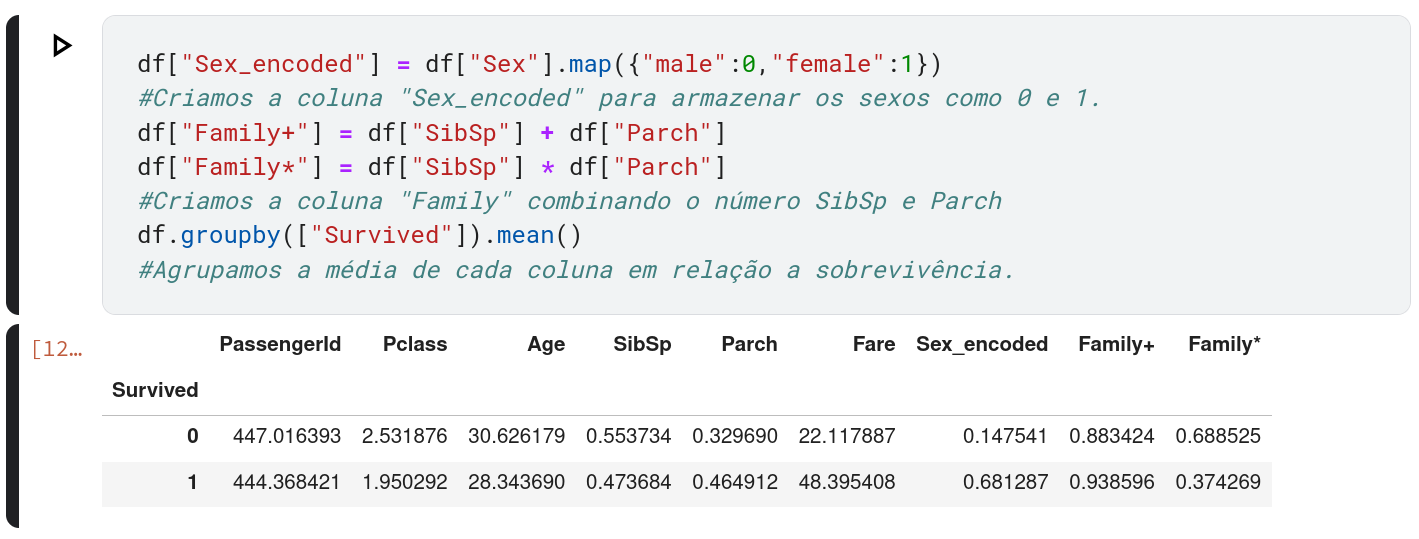
\includegraphics[width=\textwidth]{Figures/df.groupby.png}
\caption{\label{df.groupby}Agrupando cada coluna em média de acordo com a sobrevivência.}
\end{figure}

\begin{figure}[H]
\centering
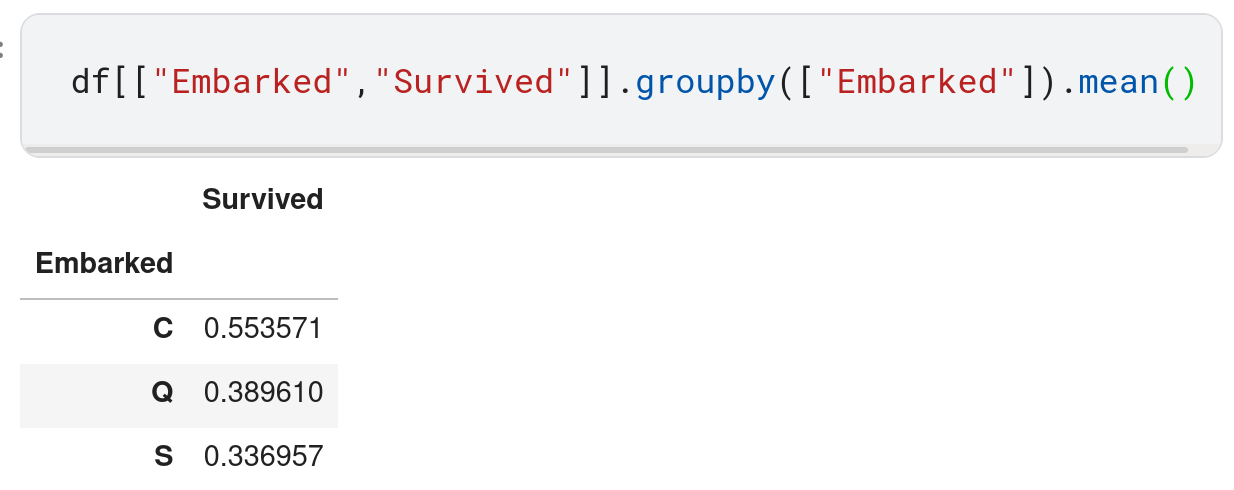
\includegraphics[width=\textwidth]{Figures/embarked.png}
\caption{\label{embarked.groupby}Agrupando a sobrevivência de acordo com os portos de embarque.}
\end{figure}

A partir dela podemos constatar que a média de classe, sexo e custo da passagem foi bem diferente entre os que sobreviveram e os que não sobreviveram, o que sugere serem variáveis importantes. O número de irmãos e cônjuges, bem como o número de pais e filhos apresentaram uma diferença mais sutil, assim como a idade. Pode ser entretanto que haja alguma relação de grupos dessas \emph{features} com a sobrevivência, conforme observamos na Figura \ref{age.hist} ao compararmos os histogramas das idades dos sobreviventes com o histograma das idades das vitimas. 
Também podemos observar nas Figuras \ref{family.groupby} e \ref{df.groupby.plot} a existência de algum padrão de sobrevivência de acordo com a quantidade de parentes a bordo. 
\begin{figure}[H]
\centering
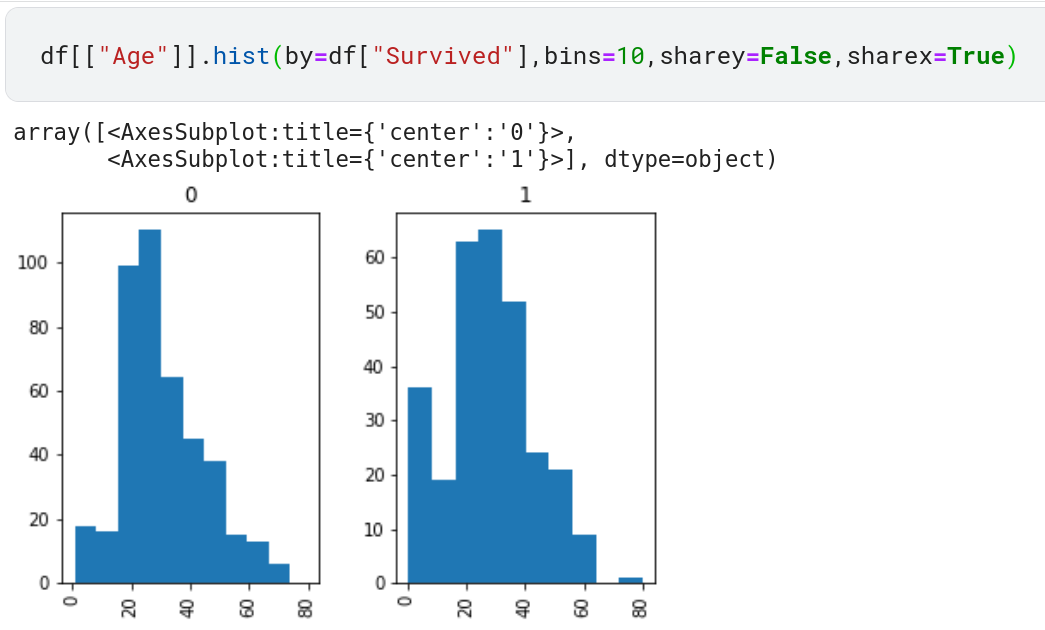
\includegraphics[width=\textwidth]{Figures/age.hist.png}
\caption{Histograma das idades dos sobreviventes e das vítimas.}
\label{age.hist}
\end{figure}

\begin{figure}[H]
\centering
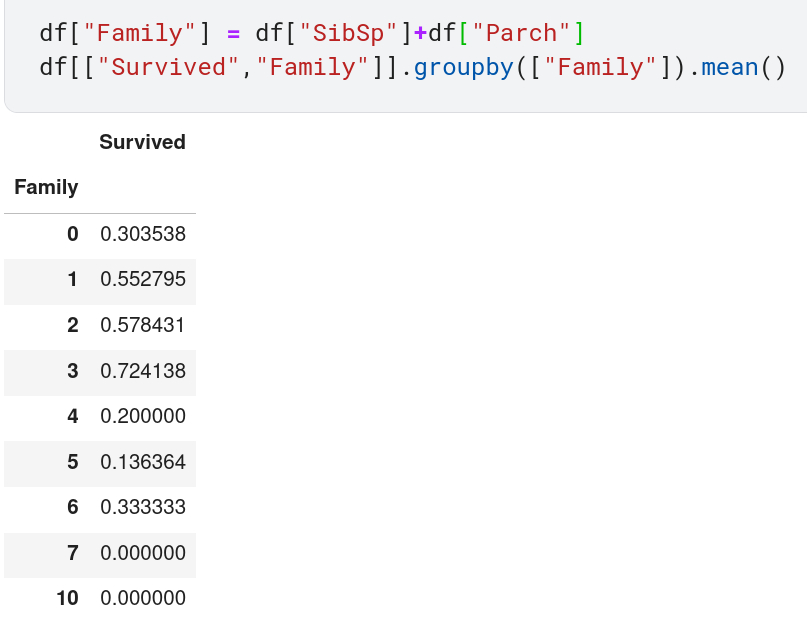
\includegraphics[width=\textwidth]{Figures/family_groupby.png}
\caption{\label{family.groupby}Índice de sobrevivência para cada quantidade de parentes a bordo.}
\end{figure}
\begin{figure}[H]
\centering
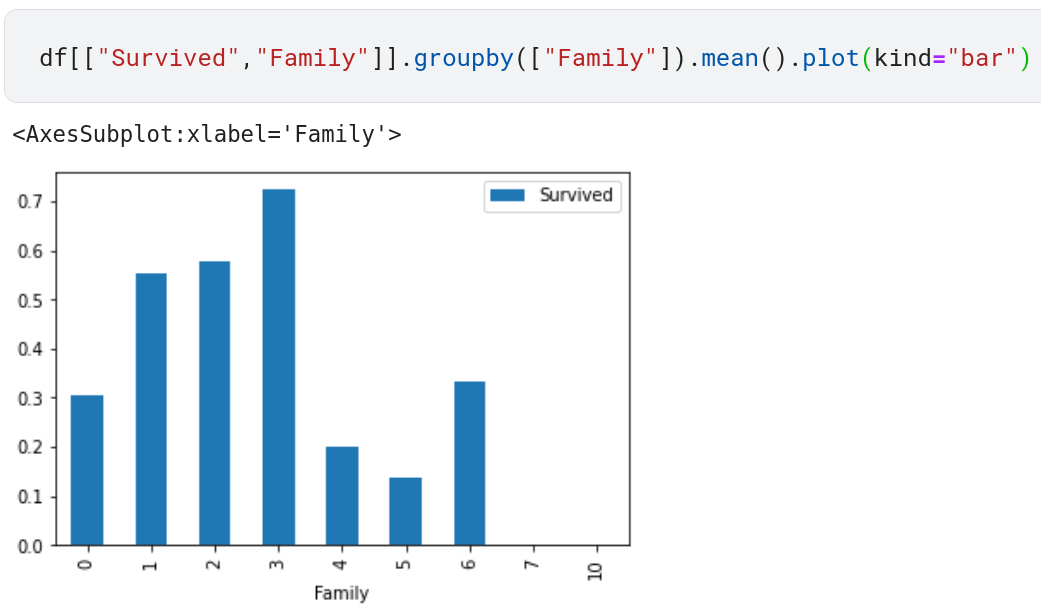
\includegraphics[width=\textwidth]{Figures/family_survivor_plot.png}
\caption{\label{df.groupby.plot}Gráfico do índice de sobrevivência para cada quantidade de parentes a bordo.}
\end{figure}

Assim, concluímos o seguinte:
\begin{itemize}
\item Removeremos as colunas: \\textit{PassengerId, Name, Ticket} e \\textit{Cabin}. 
\item Pclass já pode ser utilizada conforme se encontra.
\item Modificaremos a feature Sex codificando os valores male e female para 0 e 1 respectivamente. 
\item Completaremos os valores faltantes da Age considerando a mediana da o sexo e a classe do passageiro do passageiro. 
\item Criaremos a feature Family combinando Parch e SibSp e a codificaremos numericamente. 
\item Fare, assim como Pclass já está pronta para ser utilizada. 
\item Codificaremos os portos em Embarked.
\end{itemize}

Finalmente, uma vez que estabelecemos um plano, podemos aplicá-lo ao nosso dataframe \textsc{df}. Um ponto muito importante é que devemos estruturar as transformações de modo que possam ser aplicadas tanto nos dados de treino quanto nos dados que o modelo receberá em produção. Desse modo, obtemos nosso dataset tratado, conforme temos na Figura \ref{wranglin.results}.

\begin{figure}[H]
\centering
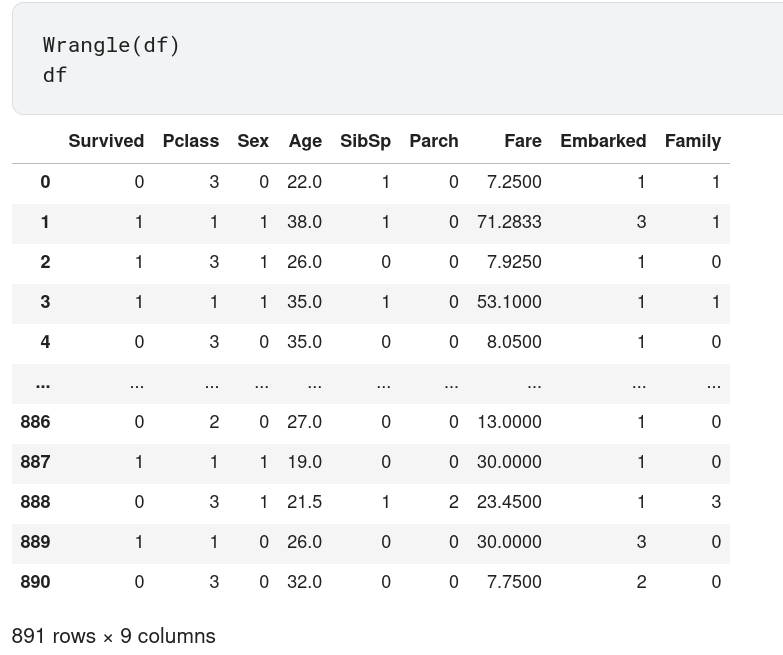
\includegraphics[width=\textwidth]{Figures/wrangle_results.png}
\caption{\label{wranglin.results}Aplicação da função \emph{Wrangle()} para preprocessar os dados de treinamento.}
\end{figure}

\subsection{Aprendizado de Máquina}
\subsubsection{Conceitos Principais}
No modelo \cite{BATON}, após o macroprocesso de \\textit{Preparation} temos o macroprocesso \\textit{Analysis}. Dessa forma, essa etapa que chamamos de \\textit{Aprendizado de Máquina} é equivalente aos seguintes processos da pipeline:
\begin{itemize}
\item \textbf{Modeling}: aplicar técnicas computacionais e estatísticas para derivar informação que oriente possíveis ações a partir dos dados. 
\item \textbf{Verification}: é o processo avaliativo para confirmar a robustez dos resultados do código e dos modelos. É interessante notar que tem crescido a importância também de considerar a transparência e imparcialidade (fairness) dos processos de dados. 
\item \textbf{Interpretation}: processo de compreensão dos resultados, da exploração e do modelo no que diz respeito as suas aplicações no mundo real.
\end{itemize}

As principais ferramentas desse etapa no ecossistema Python são:
\begin{itemize}
\item Bibliotecas Pandas e NumPy utilizadas, assim como na etapa anterior, para manipulação de tabelas e operações com colunas.
\item \textit{Scikit Learn}: é a principal biblioteca para aprendizado de máquina em Python. Podemos utiliza-la para facilmente criar modelos dentro dos diversos tipos oferecidos. Ela também oferece ferramentas para suportar todo o processo de treiná-los, avalia-los, ajustá-los e utilizá-los. Além ser open source e de oferecer diversas outras funcionalidades como a criação de pipelines de processamento automatizado. [citar a própria página oficial do projeto] 
\end{itemize}

Nesse contexto, quando falamos de \\textit{Aprendizado de Máquina} (ML), nos referimos a modelos preditivos que "aprendem" a partir de dados. Normalmente, os modelos encontram as relações e correlações entre colunas de uma tabela. Nesse sentido, podemos definir um modelo como a especificação de uma relação matemática ou probabilística entre variáveis,  \cite{SCRATCH} \cite{PRINCIPLES}.

\cite{PRINCIPLES} Ressalta as seguintes premissas universais a todos os modelos de ML:
\begin{itemize}
\item Os dados de entrada devem ser limpos e pré processados. Poucos modelos toleram dados sujos, com valores faltantes ou variáveis categóricas. Nesse sentido, parte importante da preparação dos dados envolve lidar com essas questões.
\item Em geral, são muito sensíveis a dados ruidosos. 
\item Cada linha da tabela representa uma única observação do ambiente que tentamos modelar. 
\item  Deve existir alguma relação entre variáveis.
\item Modelos são geralmente considerados semi-automáticos, isto é, necessitam que humanos tomem decisões. Seu output é normalmente uma sequência de números. Um ser humano é necessário para analisar esses resultados com a perspectivas adequadas e comunica-los.
\end{itemize}

Nesse sentido, \cite{SCRATCH} elenca os seguintes conceitos fundamentais à modelagem de dados:
\begin{itemize}
\item Overfitting e Underfitting: é a medida do quanto o modelo é capaz de aprender e generalizar determinado conjunto de dados. Overfitting ocorre quando o modelo "decora" os dados de treino, portanto ele tem um excelente rendimento com dados conhecidos e péssimo com dados novos. Underfitting quando ele não aprende o suficiente.
\item Bias-Variance trade off: analoga ao over e underfitting, um modelo com Bias alta performa mal até mesmo nos dados de treino (underfitting), enquanto uma variança alta significa que dados diferentes levariam a modelos muito diferentes, o que corresponde ao overfitting.
\item Correctness: Existem diversas métricas para se avaliar um modelo. Normalmente se utiliza Acurácia,  Precision and Recall, muitas vezes a sua média harmônica denominada F1-score. 
\item Feature selection, extraction e engineering: um dos conceitos mais importantes de um modelo são as suas features, a seguir detalhamos seus principais conceitos e técnicas.
\end{itemize}

\subsubsection{Feature Engineering} \label{feature-Eng}
O objetivo do Feature Engineering é aumentar a performance preditiva do modelo, diminuir a necessidade computacional e de dados, e finalmente melhorar a interpretabilidade dos resultados. Nessa sessão abordamos os principais fundamentos, e a práticas na preparação das features de um modelo. 

Nesse sentido, \cite{SCRATCH} ressalta os seguintes pontos centrais:
\begin{itemize}
\item Features são quaisquer inputs do nosso modelo. 
\item Quando nossos dados têm poucas features o modelo tende ao underfit. Do mesmo modo que o excesso de features faz com o que o modelo overfite. 
\item Existem três tipos principais: booleano (0 ou 1), numérico e categórico (uma escolha dentro um conjunto discreto de opções).
\item O tipo das features pode restringir o tipo de modelo que pode ser usado. Como por exemplo os modelos de regressão requererem dados numéricos, enquanto árvores de decisão conseguem lidar tanto com dados numéricos quanto categóricos.
\end{itemize}

Dentre as práticas mais importantes nesse processo de construção das features de um modelo podemos citar:
\begin{itemize}
\item Compreender as features, estudar o dataset e sua documentação, pesquisar o problema a ser solucionado tanto com profissionais da área quanto por meio de livros e artigos. Relações numéricas entre features são normalmente expressas por fórmulas matemáticas. Frequentemente as descobrimos quando pesquisamos a área do problema.
\item Estudar outras soluções para problemas similares, ou anteriores.
\item Usar a visualização de dados. A visualização muitas vezes pode revelar patologias em uma distribuição, ou inspirar possíveis simplificações para relações complicadas, ou ainda sugerir algum tipo de transformação como por exemplo aplicar uma função logarítmica. 
\item Podemos utilizar uma função para medir a relação de determinada feature com a variável alvo e desse modo rankea-las para facilitar a busca das  features mais interessantes. Mutual Information é um exemplo de métrica utilizada nesse sentido, semelhante a correlação estatística, ela tem a vantagem de conseguir medir qualquer relação, não apenas linear entre variáveis. 
\item A utilidade de uma feature, entretanto, é diretamente proporcional a capacidade do modelo aprender a relação dela com a variável alvo. Desse modo, mesmo features com alto índice de relação com a variável alvo, podem precisar serem transformadas para expor ao modelo a sua associação a variável alvo. Quanto mais complexa a combinação, mais difícil para o modelo aprender a relação.
\end{itemize}

Além das práticas podemos citar as seguintes principais técnicas para abordar esse processo:
\begin{itemize}
\item Aplicação de uma potência, raiz, ou transformar valores absolutos em percentual ou proporções
\item Normalização. Isto é, deslocar a distribuição dos dados de modo que sua média seja zero e escalar seus valores de modo que seu desvio padrão seja unitário. 
\item Criação de uma feature de contagem. Podemos agregar o número de fatores de risco, o número de ingredientes, etc.
\item Frequentemente temos features complexas que podem ser separadas em features menores, como números de telefone (operadora e número), endereço (rua, cidade, país). Da forma semelhante podemos ter features que poderiam ser combinadas como modelo e marca de carro, ou tipo e nível de um seguro.
\item Group Transforms. Podemos usar groupby para criar features como "média salarial no estado daquela pessoa", ou "Proporção de filmes lançados em determinado dia da semana, por gênero", ou "frequencia que o estado aparece no dataset"
\end{itemize}

\subsubsection{Principais modelos}
Apesar de existirem muitas classificações, modelos são geralmente divididos entre (\cite{SCRATCH,PRINCIPLES}):
\begin{itemize}
\item Supervisionados: são treinados com dados classificados, para fazer predições sobre novos dados não-classificados. 
\item Não-supervisionados: não consideram nenhuma classificação, e sim busca agrupar os dados. 
\end{itemize}

É importante considerar as características de cada tipo de modelo ao criar features para eles:
\begin{itemize}
\item Modelos lineares naturalmente aprendem somas e diferenças, mas não conseguem aprender nada mais complexo.
\item Razões são normalmente difíceis para a maioria dos modelos, logo criar features com combinações de razões frequentemente levam a ganhos de performance.
\item Modelos lineares e redes neurais geralmente funcionam melhor com features normalizadas. Modelos de árvores normalmente não apresentam tanto ganho de performance ao escalar os valores das features para valores próximos de zero (normalizar).
\item Modelos de árvores podem aprender quase qualquer combinação de features, mas quando uma combinação é particularmente importante, pode ser benéfico criar uma feature explicita, especialmente quando temos dados limitados.
\item Contagem são especialmente úteis para modelos do tipo árvore. Isso porque esses modelos não tem uma forma natural de agregar informação entre muitas features de uma vez.
\end{itemize}

Nesse projeto buscamos utilizar os modelos mais representativos que se adequassem ao problema apresentado\cite{vanderplas2016python,aurelien2017hands}. Gostaríamos de nos aprofundar nos mecanismos de cada um deles em pesquisas futuras. Utilizamos os seguintes modelos:
\begin{itemize}
\item Logistic Regression
\item Deciosion Tree Classifier
\item Random Forest Classifier
\item KNN
\item Suppor Vector Classifier
\end{itemize}


\subsubsection{Titanic}
A partir do que foi visto na teoria, construímos uma estrutura para criar os cinco modelos estudados, automaticamente treiná-los e avaliá los com os dados preprocessados. Desse modo, encontramos os seguintes resultados que serão apresentados na Figura \ref{ml.results}.
\begin{figure}[H]
\centering
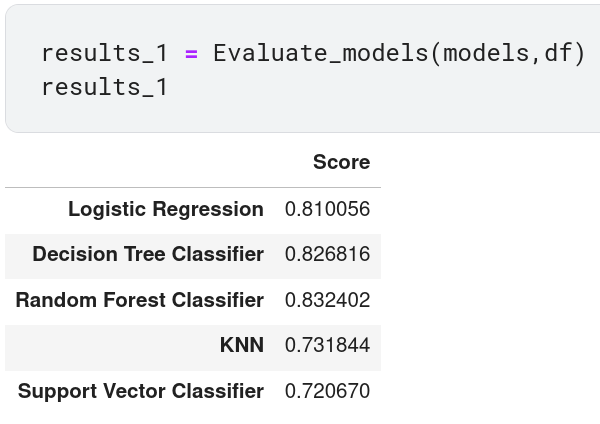
\includegraphics[width=\textwidth]{Figures/results_1.png}
\caption{\label{ml.results}Score dos diferentes modelos de Aprendizado de Máquina.}
\end{figure}

Como pode-se observar, modelos do tipo árvore foram os que melhor desempenho tiveram; seguidos da regressão logística, e finalmente os modelos não-supervisionados apresentaram o pior desempenho.

Após essa observação, aplicamos a técnica de normalização que vimos na seção \ref{feature-Eng}, em nossas features \textsc{Age} e \textsc{Fare} conforme mostrado na Figura \ref{normalized}. O resultado experimental confirma o que estudamos: modelos baseados em árvore e regressão logística são menos sensíveis à normalização. Constatamos na Figura \ref{ml.results2} que de fato, sua pontuação não foi alterada enquanto os modelos não supervisionados apresentaram uma melhora considerável de desempenho. 

\begin{figure}[H]
\centering
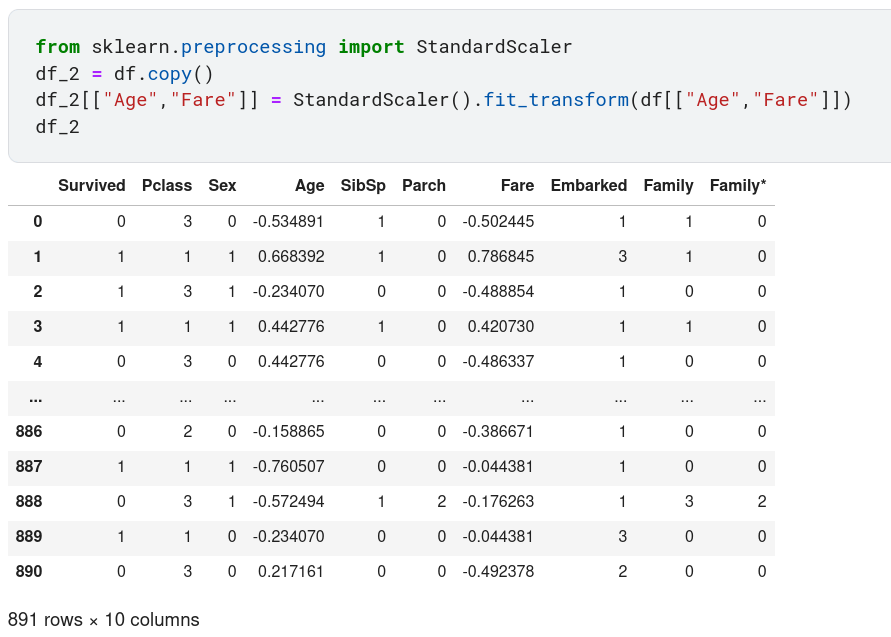
\includegraphics[width=\textwidth]{Figures/normalized.png}
\caption{\label{normalized}Comparação da performance após a normalização de Age e Fare.}
\end{figure}
\begin{figure}[H]
\centering
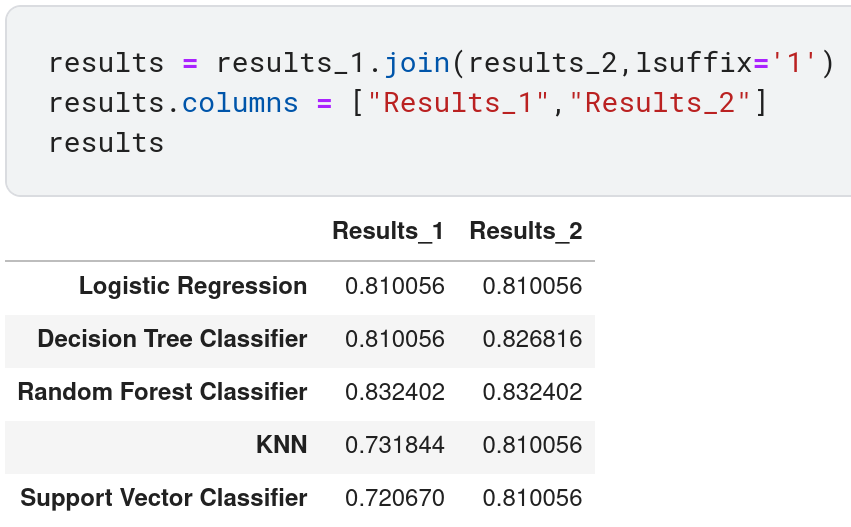
\includegraphics[width=\textwidth]{Figures/results1_2.png}
\caption{\label{ml.results2}Comparação da performance após a normalização de Age e Fare.}
\end{figure}
Assim, concluímos que modelos de arvore funcionaram melhor, especialmente o Random Forest. Também observamos que os tripulantes mais abastados, mulheres, crianças e idosos tiveram mais chance de sobreviver.

\subsection{Data Visualization}
O artigo \cite{BATON} busca definir a ciência de dados e seu modelo de trabalho justamente tendo em vista localizar o papel da visualização de dados dentro desse campo. Concluindo que apesar de pouco reconhecido entre cientistas de dados, o uso da visualização percorre a maior parte das etapas de um projeto de dados. 

Nesse ano de trabalho, a visualização de dados foi usada em diversos momentos das duas etapas anteriores (Análise de Dados e Aprendizado de Máquina), além da apresentação dos resultados. Tanto os gráficos que utilizamos, quanto as tabelas, e até todas as ferramentas, como o próprio conceito de notebook de código estão intimamente entrelaçados com conceitos de apresentação visual de informação, comunicação, arte e fundamentalmente design. 
Assim, um seguimento muito importante desse nosso primeiro ano envolve nos aprofundarmos e mapearmos essa área tão rica e diversa. 

\subsection{Deployment}
\subsubsection{Titanic}
Conforme apresentamos na metodologia, essa etapa final de um projeto de dados envolve transferir a solução construída para o seu ambiente final. Desse modo, para o Titanic, criamos e submetemos o arquivo final com as predições de nosso modelo para cada passageiro presente nos dados do arquivo test.csv. Tais dados são 418 novas entradas para as mesmas 11 colunas de features que o nosso arquivo de treino. Assim, após o treinamento dos modelos, aplicamos o modelo de melhor performance para predizer a sobrevivência desses 418 passageiros. 

Nossa solução obteve o score de aproximadamente 78\% no Kaggle, como mostra a Figura \ref{kaggle.score}. Tal desempenho é compatível com os números encontrados na validação do modelo. Assim, uma vez submetido, podemos permitir que nosso caderno seja acessível ao público. \footnote{https://www.kaggle.com/danielbritodossantos/dbs97-titanic}

\begin{figure}[H]
 \centering
 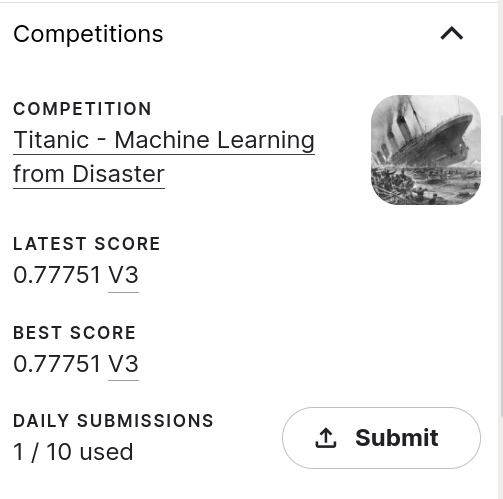
\includegraphics[width=\textwidth]{Figures/Score.png}
 \caption{\label{kaggle.score}Pontuação final no Kaggle.}
\end{figure}
\subsubsection{Aprofundamentos}
Considerando que a entrega final de um projeto de dados pode ser um relatório, o deployment de um modelo ou de uma infra-estrutura computacional, como vimos na seção \ref{principais.conceitos}, nesse ano demonstramos a entrega de um modelo, neste relatório também podemos encontrar aspectos de um relatório de dados.

Entretanto, o deployment de infra estrutura envolve um considerável corpo de conhecimentos. Portanto, nesse ano identificamos os contornos dessa área, esperamos nas próximas etapas desenvolver seus principais conceitos. Tais como redes, aplicações e serviços web, técnicas para armazenagem de funções e modelos treinados, frameworks dentre outras. 

\chapter{Conclusão}
Assim, podemos afirmar que nosso objetivo principal foi concluído. Uma vez que foi possível percorrer um vasto terreno, compilar diversas técnicas e conceitos, compreender a sua estrutura e como muitas dessas partes dialogam entre si, além de encontramos diversas oportunidades de aprofundamento. 

Assim, concluímos citando Tukey \cite{FoDA} em tradução livre:
\begin{quote}
O futuro da [ciência de dados] pode envolver grande progresso, superar dificuldades reais, e prestar um grande serviço para todos os campos de ciência e tecnologia. Isso vai acontecer? Depende de nós, de nossa vontade de percorrer o caminho difícil dos problemas reais ao invés do caminho suave das premissas irreais, critérios arbitrários e resultados abstratos sem impacto no mundo real. Quem aceita o desafio?
\end{quote}

\chapter{Perspectiva de continuidade}
A partir da construção dos fundamentos da ciência de dados, identificamos diversas oportunidades de desenvolvimentos futuros, principalmente nas áreas de Data Visualization, Bancos de Dados e Aprendizado de Máquina. Especialmente na possibilidade de nos aprofundarmos em seus corpus de conhecimento e aplicá-los em projetos reais. 
\chapter{Participação em congressos e trabalhos publicados ou submetidos e outras
atividades acadêmicas e de pesquisa}

Também apresentamos os certificados dos minicursos oferecidos pela plataforma Instituto de Tecnologia e Sociedade e Coursera  nas figuras \ref{Google} \ref{Design} e \ref{Direitos}.

\begin{figure}[h!tbp]
  \centering
  \begin{minipage}[b]{0.7\textwidth}
    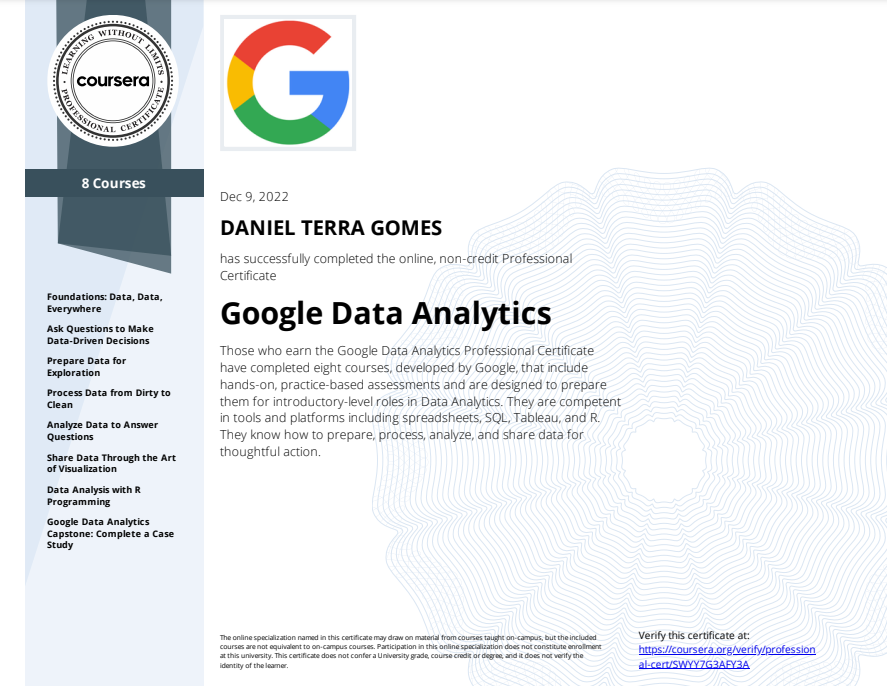
\includegraphics[width=\textwidth]{Figures/google.png}
    \caption{\label{Google} Certificado de conclusão do curso Google Data Analytics.}
  \end{minipage}
    \hfill
    
  \begin{minipage}[b]{0.7\textwidth}
    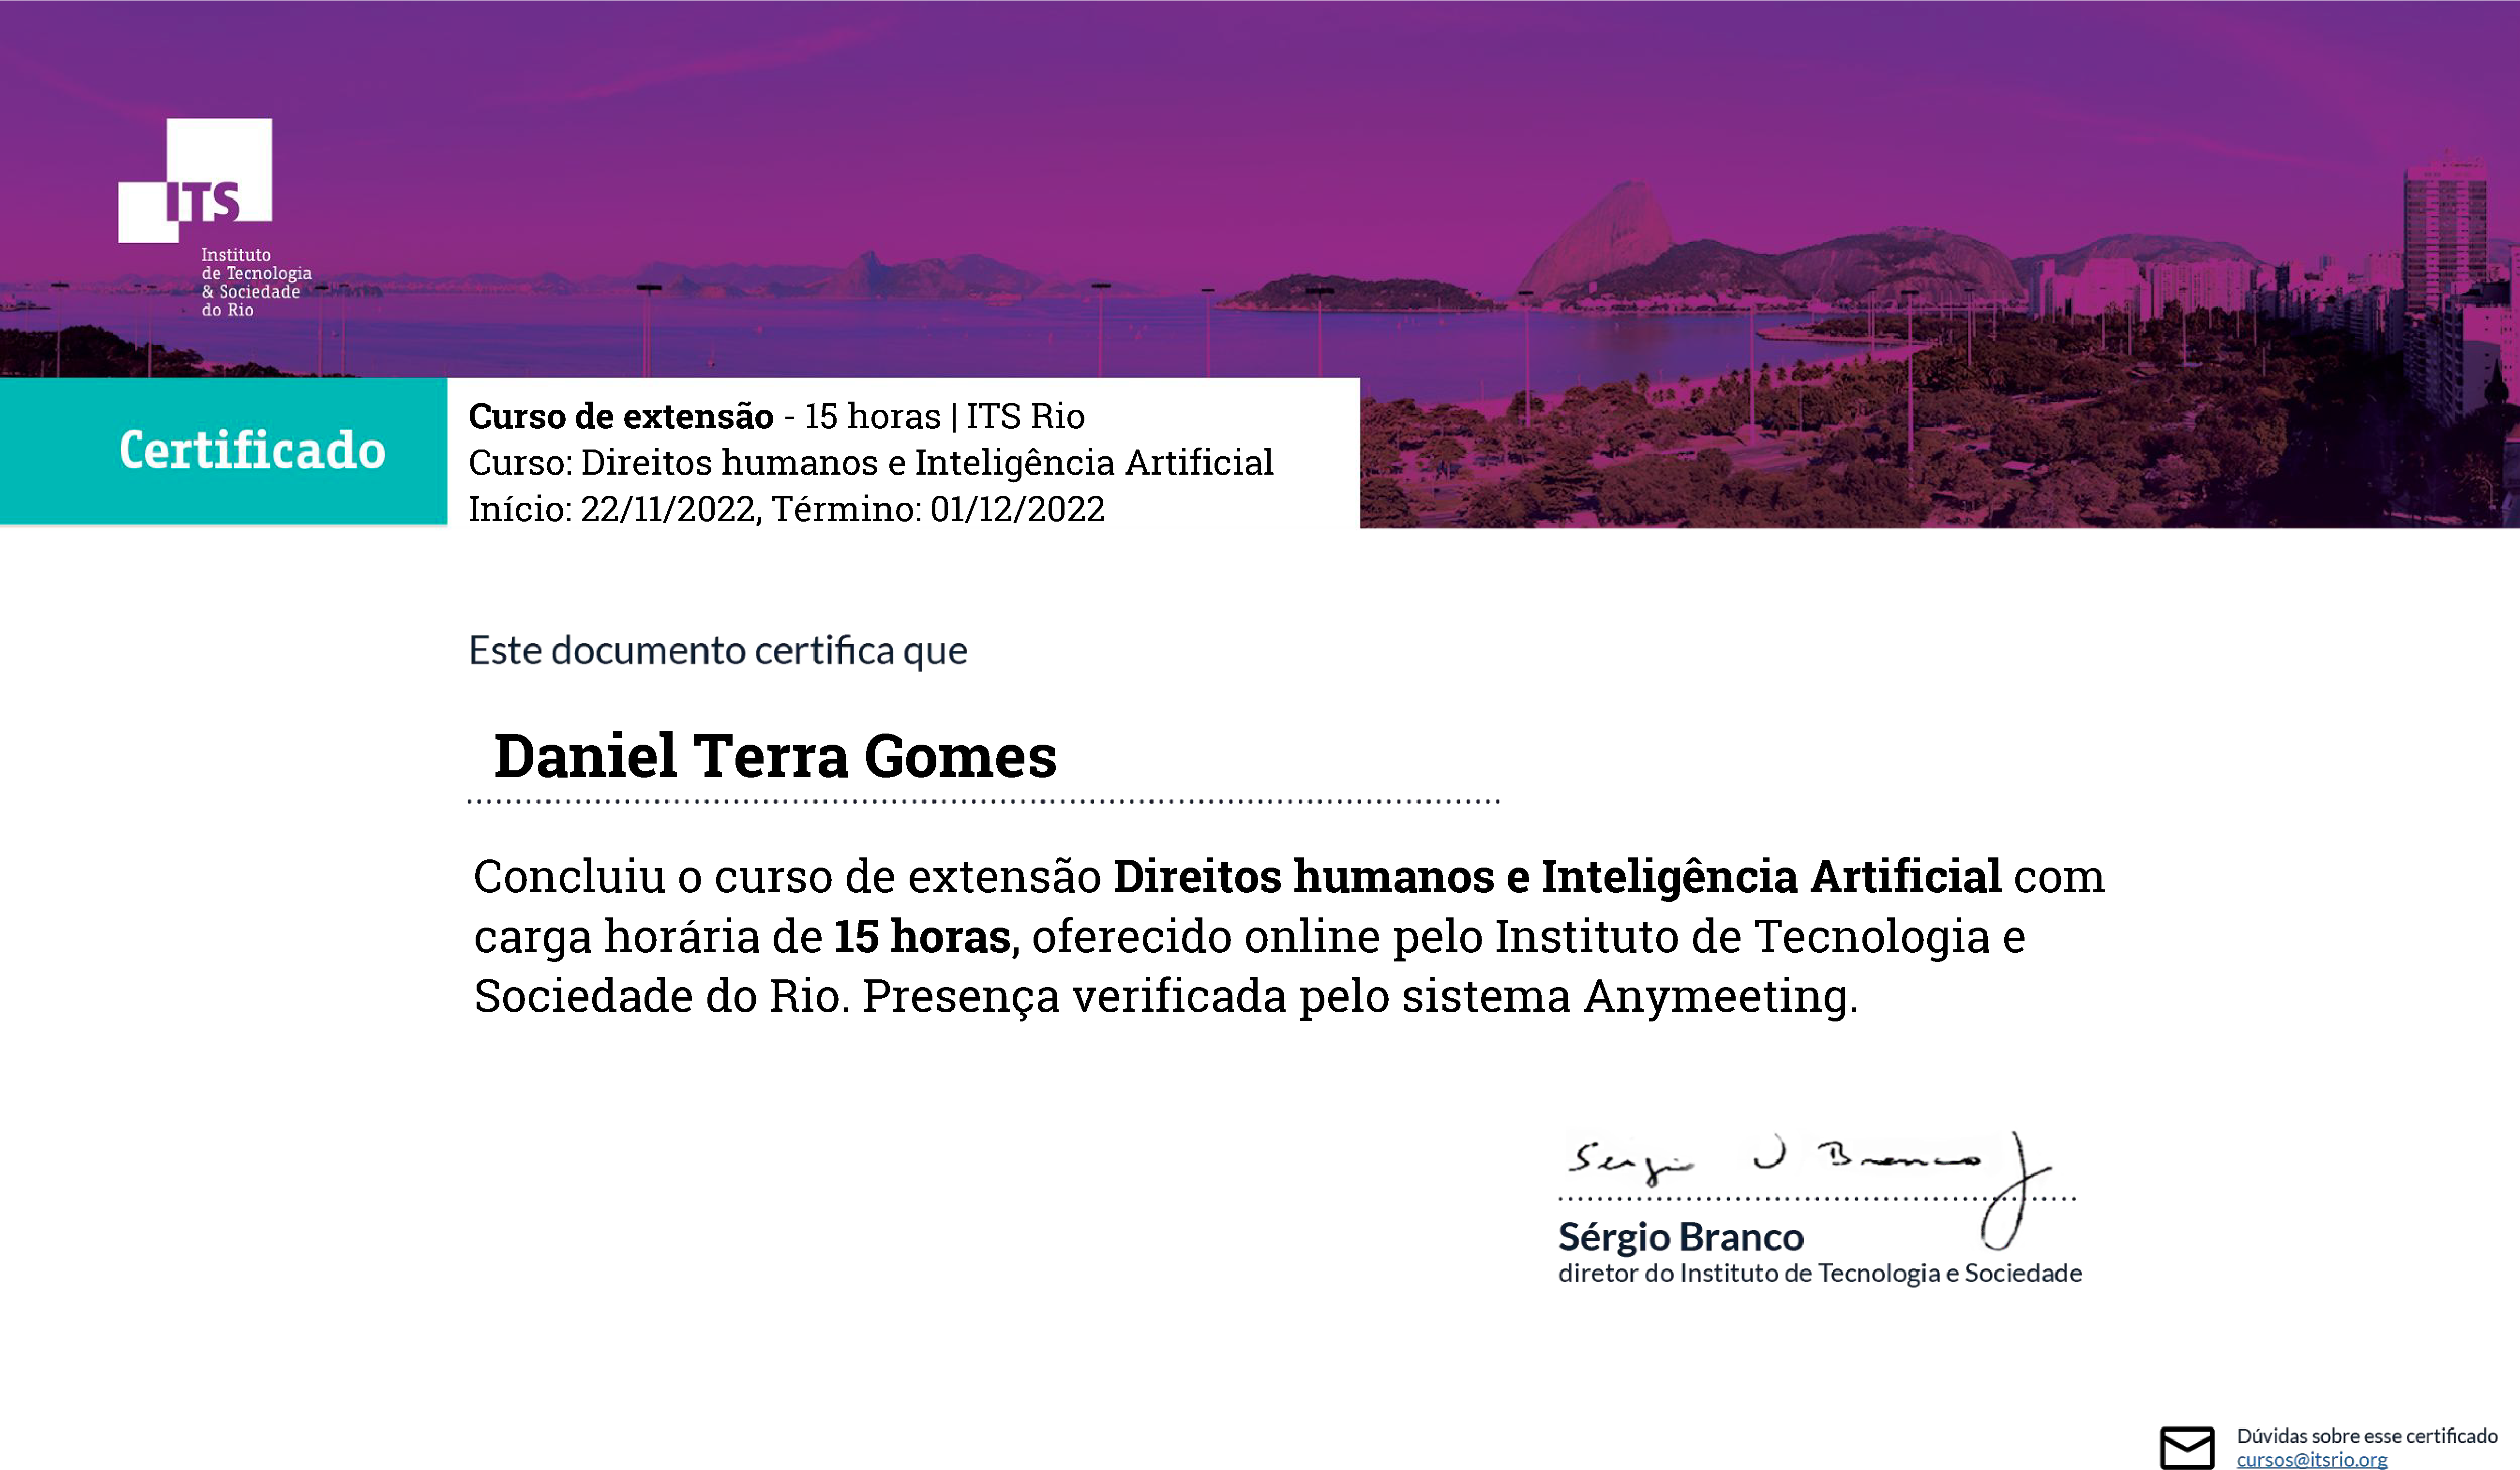
\includegraphics[width=\textwidth]{Figures/its1.pdf}
    \caption{\label{Design} Certificado de conclusão ao curso Design for Privacy.}
  \end{minipage}
\end{figure}
\begin{figure}[h!tbp]
  \centering
  \begin{minipage}[b]{0.7\textwidth}
    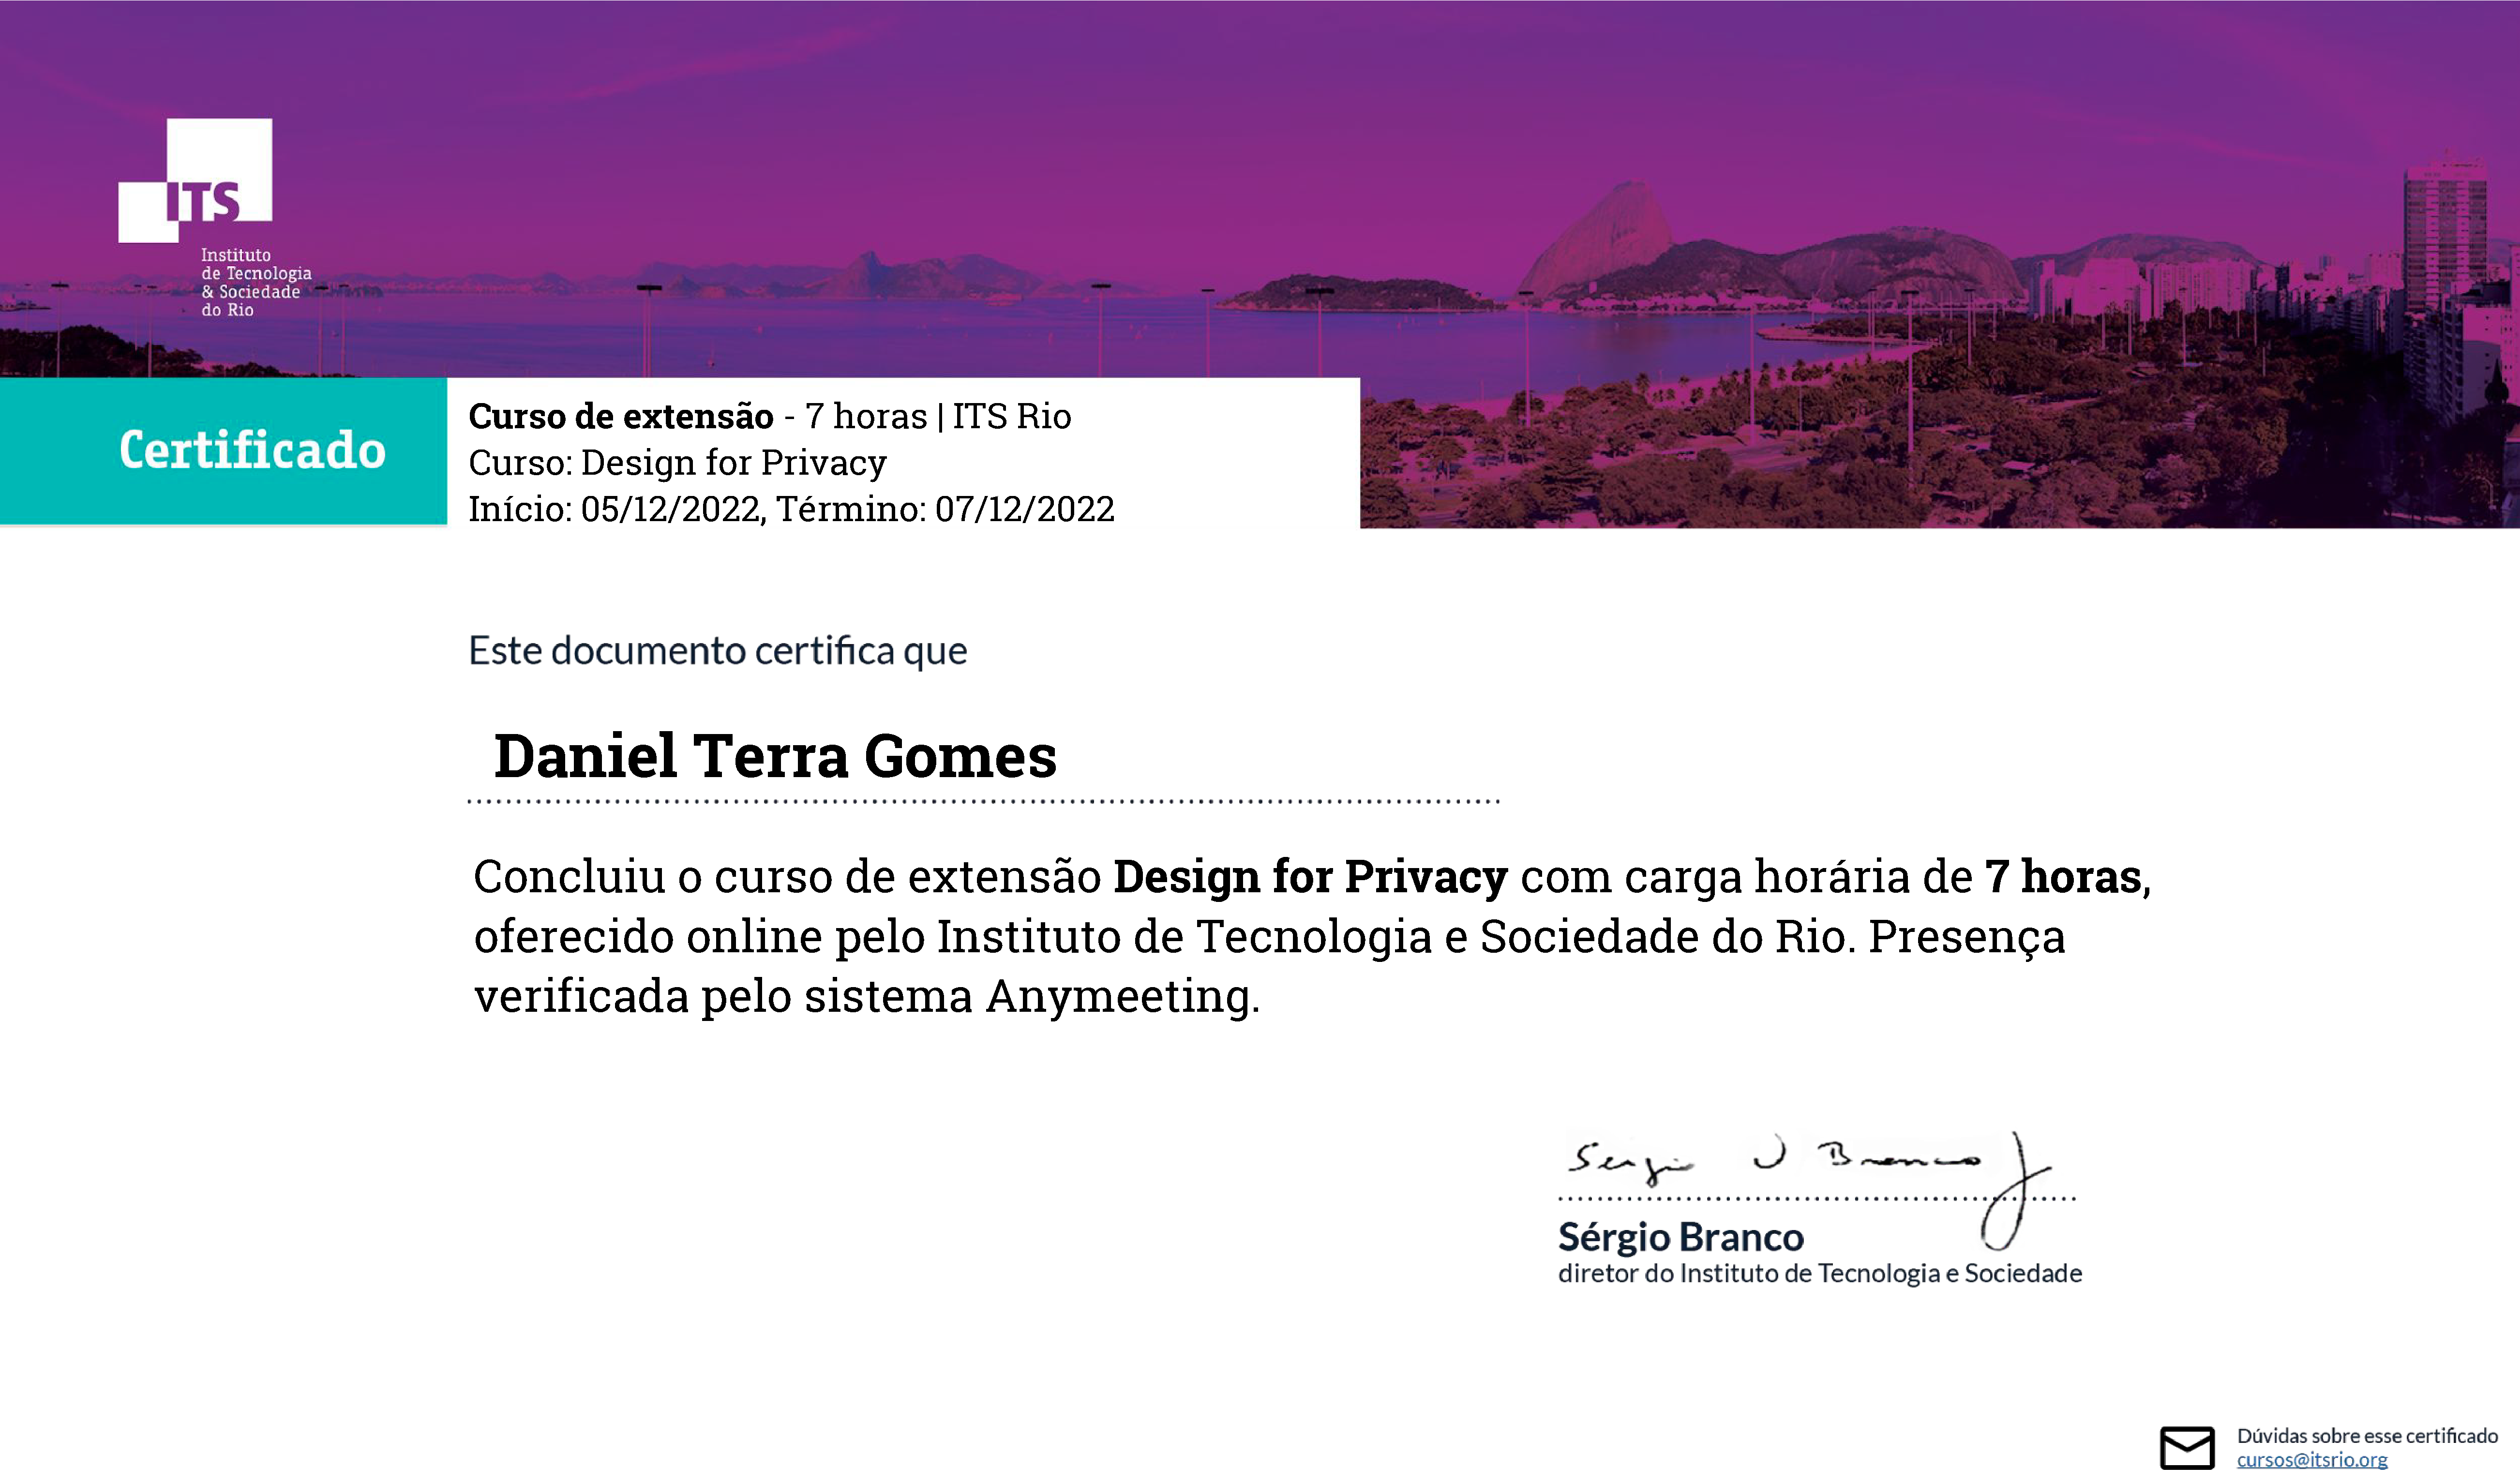
\includegraphics[width=\textwidth]{Figures/its2.pdf}
    \caption{\label{Direitos} Certificado de conclusão ao curso Direitos humanos e Inteligência Artificial.}
  \end{minipage}
 
\end{figure}


\chapter{Datas e assinaturas}
\section{Data e assinatura do bolsista (assinatura digitalizada)}


\begin{figure}[H]
 \centering
 
\includegraphics[width=0.4\textwidth]{Figures/Assinatura1.2.png}
 %\caption{\label{kaggle.score}Pontuação final no Kaggle.}
\end{figure}
\center24/01/2022

\section{Data e assinatura do orientador (assinatura digitalizada)}


\begin{figure}[H]
 \centering
 
\includegraphics[width=0.4\textwidth]{Figures/assinatura_annabell.png}
 %\caption{\label{kaggle.score}Pontuação final no Kaggle.}
\end{figure}
\center 28/01/2022

